

\section{ABSTRACT}
Personalization approaches seek to estimate user preferences in order to recommend content or social network connections, or to serve personalized advertisements to users. Such approaches are being increasingly adopted by organizations to build customized personalization applications. Leveraging the growing popularity of web videos for such approaches necessitates the ability to classify web videos into application-specific categories since different applications are interested in different aspects of the user preferences. A key requirement of supervised classification models to address this is the availability of training videos labeled to the arbitrary application-specific categories. In order to address this requirement, we propose a completely automated framework to obtain training web videos for arbitrary categories, which does not rely on any manual labeling of videos. This is achieved by utilizing keywords to retrieve training videos, thereby simplifying the problem of obtaining training videos to the problem of selecting keywords to retrieve them. We show that there are two opposing objectives (proximity and diversity) that need to be considered while developing such keyword selection techniques. We propose two efficient approaches (LCPD and AAO) and study the trade-offs between them, with respect to performance and the human input required to tune parameters of the approach. Through experiments over several sets of categories, we demonstrate the feasibility of the automated framework to select training videos for application-specific categorization. We also show that the proposed approaches lead to a substantial improvement in the performance of classification models, as compared to other automated methods. 



%% Input other tex files. Begin. %% 
\section{Introduction}
\label{sec:intro}
Over the past few years, there has been a steady rise in the number and popularity of personalization applications available on the Internet. These include applications based on personalized advertisements, content recommendation systems, social network connection suggestions, and several others, that attempt to understand the preferences of users. Personalization applications have been traditionally based on learning user preferences through queried keywords and viewed articles~\cite{mobasher2000automatic}. The last few years have also witnessed a tremendous increase in viewing and sharing of web videos (such as on YouTube\cite{Youtube}), with significant increases in unique viewers, total streams viewed, number of streams per viewer, and the time per viewer~\cite{Neilson2011}. Given their unique characteristics, web videos offer a tremendous potential for understanding user preferences.

User preferences can be inferred based on the types/categories of web videos seen. Such videos are generally organized at video sharing websites on the basis of labels that the video uploaders choose from among a set of common categories that are used by such websites. Examples of such common categories include Comedy, Music, People, Entertainment, Pets, Science, etc. On the other hand, the categories of interest to personalization applications may be arbitrary, and quite different from the above common categories. Consider a department store (such as Sears or Walmart) that might want to offer promotional coupons to buyers. Knowing whether a person (a buyer) has interest in product specific categories like fitness equipment, clothing items, or baby products would be of high interest to the department store, as compared to knowing whether he/she is interested in the common categories mentioned above. A movie recommendation system would like to learn if a viewer prefers action, horror, or comedy movies. Categorizing viewed videos and understanding user preferences in terms of the common categories used by video sharing websites might not be useful for different personalization applications. In addition to the above observation, it should be noted that different personalization applications are interested in understanding user preferences with respect to very different sets of categories, as shown by the above examples. It is clearly not sufficient to use a common set of categories for every personalization application, as the categories of interest for one application might be irrelevant and useless for another.

This calls for techniques to classify viewed web videos, and hence estimate user preferences, in terms of any arbitrary set of categories appropriate for a given personalization application. Various modes of information (such as audio, visual, textual and social network) can be employed to assist in the classification of web videos. Classifiers employed for this task have the inherent requirement of training videos labeled to the set of categories as desired by the personalization application. Since the set of categories suitable for a personalization application might be very different from the common categories used by video sharing websites, training videos labeled according to the required set of categories are often unavailable. Our work addresses this requirement of obtaining training videos labeled as per the required set of categories, which are not necessarily the categories commonly associated with web videos. We propose a fully automated framework to obtain training videos with properties that can lead to high performance of trained classification models. To achieve the above, the proposed framework neither relies on labels associated with online videos, nor requires any manual labeling of videos. Instead, we develop approaches to select keywords based on their suitability to retrieve high quality training videos for a specified set of categories. Such a methodology requires the consideration of two opposing objective, namely proximity and diversity. In order to select the keywords, we first present a tunable approach  (LCPD) based on the Linear Combination of Proximity and Diversity. While such an approach can give good classification performance, it requires the tuning of a parameter in order to obtain optimal performance, which may require manual effort. We thus also propose an approach using Annealing based Alternating Optimization (AAO) where we balance between the two objectives such that the final solution is a trade-off between the two. Complexity, convergence and correctness of the proposed algorithms are presented, along with experiments over several sets of categories. 

\subsection{Related work} 
\label{sec:relatedwork}
We discuss below the related work on video classification. Since the keyword selection based approach requires optimizing for two objective functions, we also provide a discussion on the related work on multi-objective optimization. \\

\noindent \textbf{Video classification: }\\ 
A significant amount of work has been done to address the problem of video classification. Such work can be looked at on the basis of two dimensions -– modalities used for classification, and approaches to obtain labeled training videos.  While the focus of our work is on obtaining training videos, we first briefly describe video classification approaches in terms of modalities used, including our approach, and then discuss approaches to obtain training data, contrasting our approach from others. 

A characteristic property of web videos is that they have rich information in several modes -- audio, visual, textual, and social network being the most common ones. Methods such as \cite{song2010taxonomic,wang2010youtubecat,zhang2011improving,ramachandran2009videomule,yang2007multi} present multi-modal techniques for classification of web videos. Others such as \cite{schindler2008internet,chen2010effective} classify videos using only the audio-visual information in the videos, while \cite{chen2010web,wu2010data} approach classification of web videos by treating them as text documents. A detailed survey on video classification is provided in \cite{brezeale2008automatic}. In our work, we classify web videos on the basis of the contextual information surrounding them, such as the title, keywords, and description. This is because text-based classification approaches are computationally much less expensive than multimedia features-based classification approaches, and as shown in existing literature as well as in Section~\ref{sec:expt}, offer good classification performance.  

With respect to the approaches to obtain labeled training videos, \cite{chen2010web,wu2010data,ramachandran2009videomule}   obtain training videos that are labeled according to categories used by YouTube~\cite{Youtube}. Hence, such approaches cannot be used for classification of web videos to arbitrary set of categories, which is the focus of this chapter. Approaches such as \cite{schindler2008internet,yang2007multi,song2010taxonomic}  utilize training videos that are labeled manually. Recently, techniques have been developed \cite{wang2010youtubecat,zhang2011improving} which expand the set of training videos starting from a set of manually labeled videos. With the help of social network structure of the video sharing website, co-watched videos, or text-based classifiers, \cite{wang2010youtubecat,zhang2011improving} increase the number of training videos in a semi-supervised fashion. However, manual labeling requires human experts to go through at least a part of the video, and come up with a label. The labeling process is prone to human errors and inconsistencies, and more critically, is not scalable to large sizes of training data, especially given the enormous scale of web videos \cite{Neilson2011}. Contrary to these approaches, we propose a framework that does not require any manual effort to obtain training videos, even for any arbitrary set of categories desired by a personalization application.\\

\noindent \textbf{Multi-objective optimization: } \\
In general, for multi-objective optimization problems, there does not exist a single solution that optimizes all objectives. \cite{Marler04} surveys the different approaches that are adopted to solve multi-objective optimization problems. Certain approaches require apriori knowledge of the preferences for the different objective functions. In order to utilize these preferences, a global objective function can be defined based on the individual objective functions and by using the preferences as numerical weights, as is shown in \cite{Papalambros96,Bridgman22,Koski87}. For example, a common approach to multi-objective optimization is to combine the individual objective functions through a weighted sum method as shown in \cite{Steuer89}. 

Other works embed the notion of preferences into their methodology, for example by ranking the objective functions in the order of their relative importance \cite{YoonHwang95,Hertz94} or by modifying the bounds of the individual optimization problems \cite{HwangMasud79,Haimes71}. Such works however require the apriori knowledge of the preferences of the multiple objectives, as obtained by a human decision maker. 
%Such human involvement makes the keyword selection procedure non scalable, subjective and time consuming. 
In the context of our problem of selecting keywords to obtain training videos, such relative preferences of different objective functions is unavailable and hence these approaches cannot be applied. 

A different line of works approach multi-objective optimization problems by first obtaining a set or a representation of \textit{pareto optimal} solutions for the problem, and then employing human judgment to decide the best solution. Pareto optimal solutions are alternative solutions for the multi-objective optimization problem that are optimal in the wider sense that no other solutions in the search space are superior to them when all the objectives are considered \cite{SumanAnnealing05}. Refer to \cite{Marler04} for the mathematical definition of pareto optimality. Thus, works such as \cite{Messac02,Martinez01,Messac01} focus on finding the set of pareto optimal solutions or their representation to serve as a palette of solutions for the human decision-maker. Varying the weights given to different objective functions is a common approach to determine the pareto optimal solutions or their subset \cite{Marler04}. Such approaches however can be extremely inefficient as they require solving the weighted formulations several times \cite{Marler04}. \cite{Hansen97} works with a set of solutions searching for Pareto optimal solutions in parallel. In order to find the best candidate in the neighborhood of each current solution, the goodness is taken as the weighted average of the objective functions. The weights are dynamically updated so that unexplored regions of solution space get more preference. Certain works such as \cite{Suman05,Smith04,Bandyopadhyay08} approach the search for pareto solutions using simulated annealing framework based on an energy function for states. These energy functions are defined based on the number of solutions that dominate or are dominated by a particular solution. See \cite{Bandyopadhyay08} for a definition of domination. Such approaches require the computation of the objective functions for all or a subset of the possible solutions. While these approaches may work for certain domains \cite{Suman05,Smith04,Bandyopadhyay08}, they would be infeasible to apply to domains when the discrete solutions are subsets of a larger set and thus the number of solutions is extremely large. As shown in Section~\ref{sec:aao}, for our problem of selecting keywords, the total number of subsets can easily be of the order of $10^{30}$ and hence such approaches would be infeasible. 
In addition, in order to use the solution in a practical setting, such approaches would still require a decision maker to choose the best solution based on his/her human judgment. Compared to these, we propose two approaches LCPD and AAO to select keywords to obtain training videos. In the former, we heuristically combine two objectives linearly and select keywords one by one without computing the objective function for all subsets. In the latter, we balance the two objective functions in our formulation (Section~\ref{sec:aao}) by alternating between algorithms that optimize for each objective individually, in a simulated annealing framework. As a result of this, for AAO it is not required to provide preferences for the individual objective functions and the approach yields a solution that is convenient trade-off between the two objective functions. We empirically demonstrate the effectiveness of the two proposed approaches for selecting keywords to obtain the training videos for a category. Furthermore for AAO, in order to reduce the time taken for the annealing based approach to converge, we propose an adaptive technique to update the annealing constraint parameter, leading to substantial reduction in the convergence time. 

This work is based on \cite{VermaWI13} which provides an approach to automatically obtain training videos. We refer to the techniques proposed in \cite{VermaWI13} as LCPD, and in addition we propose an annealing based alternating optimization approach (AAO) that does not depend on parameters that may require tuning based on human input as in \cite{VermaWI13}. Further, we propose adaptive variation of AAO to make it more efficient, and provide performance comparisons with \cite{VermaWI13}. 

For multi-class, single-label classification of web videos, we first discuss the desired properties of training videos that can lead to high performance of trained classification models. This is done in Section~\ref{sec:desiredpropdata}. Section~\ref{sec:overview} provides an overview of our framework of identifying keywords to retrieve training videos with the desired properties. It also provides a discussion on the two objective functions to select keywords. Section~\ref{sec:selectionSRK} discusses the two approaches - LCPD and AAO. Section~\ref{sec:expt} details the experimental set-up and presents performance results. Section~\ref{sec:conclusion} concludes.

\section{Desired properties of training data}
\label{sec:desiredpropdata}
\begin{figure*}[!htb]
\centering
\begin{tabular}{cc}
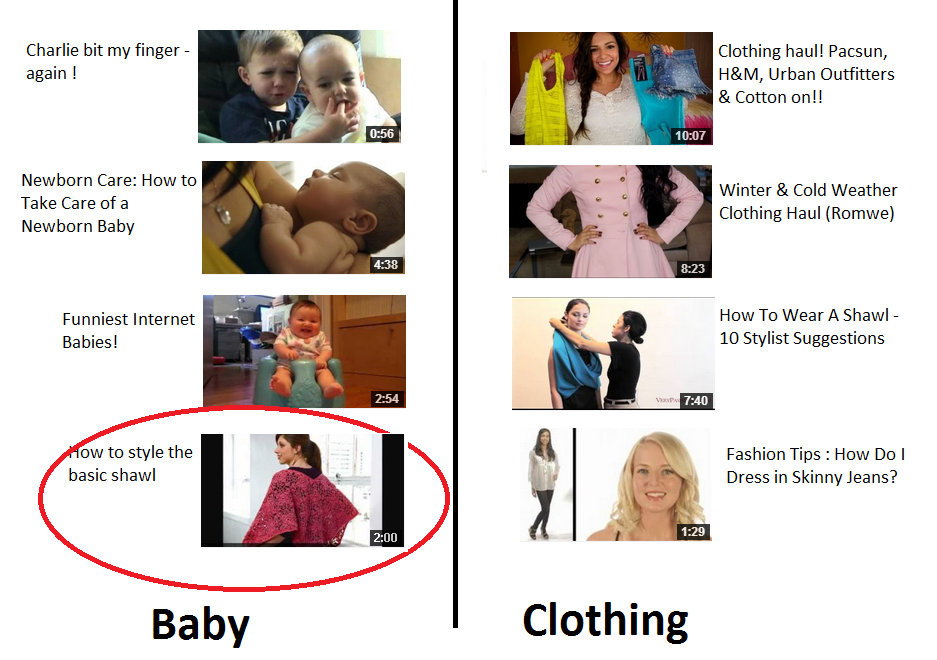
\includegraphics[width=0.45\textwidth,clip=]{TrainingData/WIfigures/mislabeled_baby_clothes_marked.png}
&
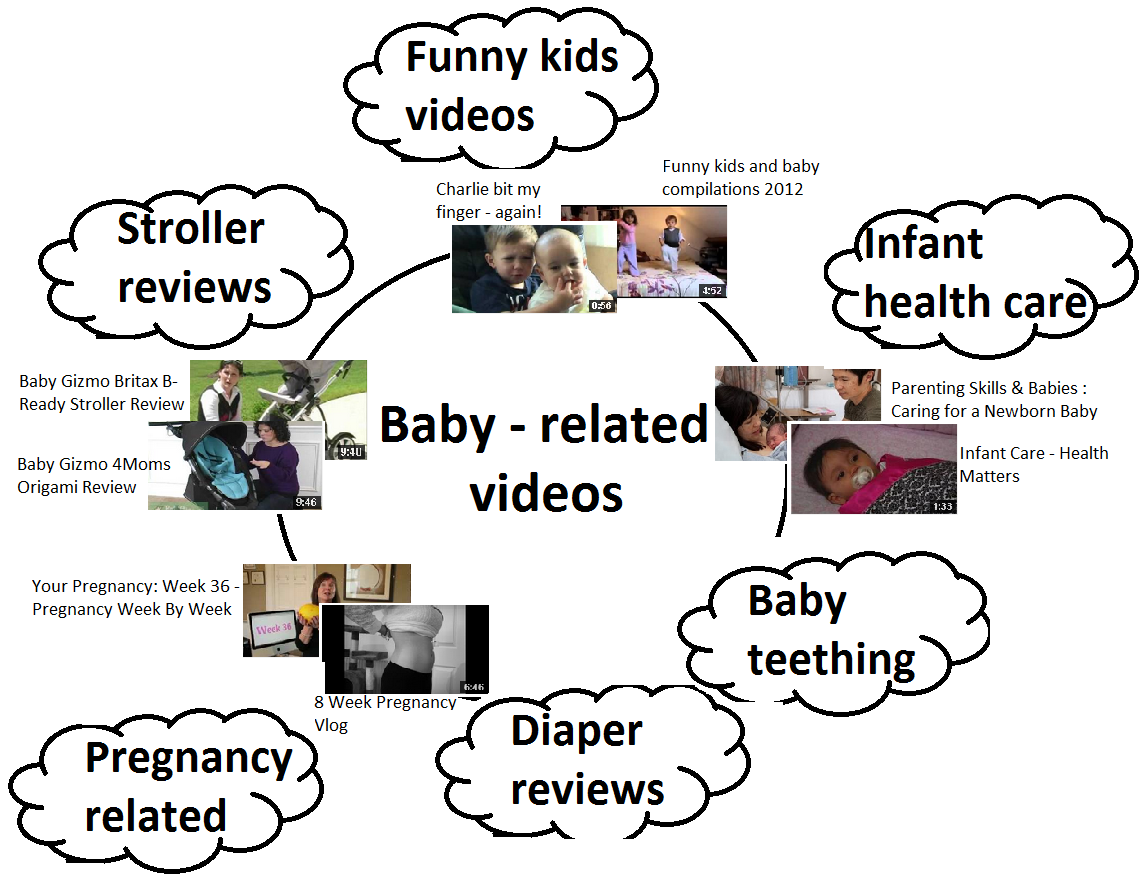
\includegraphics[width=0.45\textwidth,clip=]{TrainingData/WIfigures/diversity_baby5.png} \\ 
(a) & (b) \\ 
\end{tabular}
\caption{ \small{(a) Sample training videos for categories: \{\textit{Baby, Clothing}\}. Circled video is wrongly placed in category $Baby$, and is hence a mislabeled video. (b) Variety of video topics belonging to category $Baby$  }}
\label{fig:trainingdatapropsfigs}
\end{figure*} 
For a given classification model, a good training data would be one that has no mislabeled instances, and has high Intra-Category Diversity for each category. We discuss both factors in this section. The goodness of training data is reflected in terms of its performance on a large test set. 

In the domain of video classification, a mislabeled instance refers to a video that has the label of category $i$ as per the training data, but in actual, belong to a different category $j ( \neq i)$ as per an oracle. For instance, consider the set of categories \{\textit{Baby, Clothing, Fitness, Food}\} that a retailer may be interested in, to enable personalized promotions of the above product categories. If certain approach for obtaining training videos includes a video on $Shawls$ (as shown in Fig.~\ref{fig:trainingdatapropsfigs}(a)) to the set of training videos for $Baby$, the video would be a mislabeled video since its true label should be $Clothing$, but it has the label of $Baby$ in training data. A true label of a video is defined as the label that an oracle would assign to the video. \cite{brodley1996identifying,zhu2003eliminating} discuss techniques to identify (and eliminate) mislabeled instances from training data, for classification tasks. The performance of classification models is shown to have increased considerably after identifying (or eliminating) mislabeled videos, thus supporting that less mislabeled instances is desired in training data.  Note that the above works address the cleaning of an existing dataset whereas the problem addressed in this chapter is that of \textit{forming} a dataset by obtaining training videos with desired properties for certain given categories. In addition, in works such as \cite{brodley1996identifying} and \cite{zhu2003eliminating}, the mislabeled instances are identified as outliers in the given data, when the data itself is representative of the class in concern and captures its constituent topics. While forming a training data from real world videos retrieved using keywords, this condition is not guaranteed to be satisfied and the above techniques may not be applied. These techniques can be considered orthogonal to our work, and may further improve the training data \textit{after} it is formed using the proposed framework. 

By Intra-Category Diversity of training videos $T(i)$ of category $i$, we refer to the extent to which $T(i)$ encompasses the essence of category $i$. Let us denote Intra-Category Diversity of $T(i)$ as $div(T(i))$. In order to first intuitively motivate why high $div(T(i))$ is desired, consider the same set of categories \{\textit{Baby, Clothing, Fitness, Food}\}. Fig.~\ref{fig:trainingdatapropsfigs}(b) shows some of the various topics of videos that one would associate with the category $Baby$. A set of training videos $T_1$, having videos on \textit{Funny kids} only has less Intra-Category Diversity than a set $T_2$ of same cardinality as $T_1$ but having videos on \textit{Funny kids, Newborn care, Babysitting}, and \textit{Stroller reviews}. A classifier trained over $T_2$ is expected to have higher likelihood of categorizing correctly a test video $v$ belonging to category Baby as compared to a classifier trained over $T_1$. For instance, if a user watches a video related to review of popular strollers for infants, the model trained on $T_2$ will find it more similar to the training videos on $Baby$ than the model trained on $T_1$ will, and hence will have higher likelihood of categorizing it correctly. 

As discussed later in Section~\ref{sec:overview}, one of the shortcomings of approaches that obtain training videos without manual labeling is low Intra-Category Diversity. In such scenario, the training data of a category is skewed towards certain dominant themes within the category, and encompasses only limited topics of videos within the category. Improved techniques are hence required to obtain training videos with high Intra-Category Diversity. While it is understandable what $div(T(i))$ means, calculation of $div(T(i))$ requires knowledge of a) different topics within category $i$, and b) the extent to which these topics are covered by the training videos of category $i$. For an arbitrary set of categories, it is extremely difficult to obtain (a) and (b) above without the help of an oracle. Thus in our research, we propose the use of different techniques to obtain the degree of variation in $T(i)$ to measure $div(T(i))$. These techniques are discussed in Section~\ref{sec:overview}, and their details are provided with the respective approaches (Sections~\ref{sec:lcpd} and \ref{sec:aao}). 

The notion of diversity has been used for a variety of problems in related domains. Diversity between classification models has been discussed in works on classification model ensembles \cite{Ludmila03}. Works on summarization have used the notion of diversity between documents \cite{LiEnhanc09,ZhuNovSum13}, images \cite{KennedyGen08} and videos \cite{ShroffTMM10}. In the context of active learning \cite{WangActive11} and semi-supervised learning \cite{MisraWatch15}, diversity has been used to efficiently determine training instances to label manually. To the best of our knowledge, the use of diversity metrics in the formulation to automatically obtain training videos for classification is completely novel. 

%In Section~\ref{sec:selectionSRK}, we present numerical values for the Intra-Category Diversity and experimentally verify that an increase in Intra-Category Diversity of training data translates to improved performance of the trained classifier. 
\section{Overview of the proposed framework to obtain training videos}
\label{sec:overview}

In this section, we provide an overview of our proposed framework and approaches for identifying and selecting keywords to obtain training videos with the two desired properties described in Section~\ref{sec:desiredpropdata}. 

\indent   As discussed in Section~\ref{sec:intro}, obtaining training videos for arbitrary set of categories through manual effort is not scalable to large sizes of training data. Training videos could alternatively be obtained in an automated manner using a video search engine. This approach has also been briefly mentioned in \cite{wang2010youtubecat}, to obtain weakly labeled videos. Let $RV(K)$ represent the set of retrieved videos obtained by querying keyword $K$ in a video search engine, such as YouTube~\cite{Youtube} or Vimeo~\cite{Vimeo}. The training videos of category $i$, i.e., $T(i)$ can then be obtained simply as $RV(C_i)$, where $C_i$ is the name of category $i$. Though simple, this technique has few shortcomings. It focuses only on occurrence of the name of category and not on its semantic meaning. For example $RV(\text{`}Baby\text{'})$ mainly retrieves videos on funny kids, and music videos or other popular videos containing the word `Baby' in their title or tags. As a result, there are several mislabeled videos among training videos obtained by this approach. In Section~\ref{sec:expt}, we show how this leads to poor performance as more videos are retrieved just by the category name. At the same time, this approach does not cover the many of the semantic topics that we associate with the category of concern. For the category $Baby$, these include topics such as (in addition to funny kids,) Strollers and Bassinets reviews, Babysitting tutorials, Newborn care, Pregnancy, and several others (Fig.~\ref{fig:trainingdatapropsfigs}(b)). The Intra-Category Diversity by such an approach is hence quite low, leading to poor classifier performance. Through the proposed framework, we attempt to address the above shortcomings. We use the training videos obtained by querying name of category, i.e., $T(i)=RV(C_i)$, to train baseline classifiers to compare with our proposed approach. 

\subsection{Overview of proposed framework}
\label{sec:overviewframework}

In the proposed framework, we first collect several keywords that are related to the name of category ($C_i$). These comprise the \textbf{Candidate Keywords}. The Candidate Keywords (called candidates for brevity) can be obtained on the basis of correlation or co-occurrence with the name of the category from publicly available text documents (such as Wikipedia). Thesauri~\cite{nakayama2007wikipedia} also provide a good source for semantically (i.e., in terms of meaning) similar keywords, and can be used to obtain candidates. In addition, candidates can be obtained as related concepts or keywords from sources such as~\cite{ReverseDictionary}. The candidates can be queried in a video search engine, and their retrieved videos can be collected to obtain T($i$). However some candidates would be more useful than others, and some might be outright harmful, if used to retrieve training videos for category $i$. We discuss this in the next section. On the basis of a proposed keyword selection algorithm, we select a subset of keywords from a set of candidates for category $i$. The Selected Retriever Keywords (or SRKs) thus selected are used to retrieve training videos. If \{$K_{i,1}, K_{i,2}, ... , K_{i,L}$\}  are the SRKs for category $i$, then the training data for category $i$, i.e., $T(i)$, can be obtained as:
\begin{equation} \label{eq:trainingDataUnioneqn}
\indent T(i) = \left [ \bigcup_{j=1}^{L}RV(K_{i,j}) \right ]\cup RV(C_{i}). 
\end{equation}

If $T(i)$ were obtained as per (\ref{eq:trainingDataUnioneqn}) by selecting any arbitrary candidate keywords of category $i$ as SRKs, then $T(i)$ may not necessarily have the desired properties discussed in Section~\ref{sec:desiredpropdata}, namely low mislabeled videos, and high Intra-Category Diversity. In the next section, we discuss how we can determine the suitability of candidates to retrieve training videos with the desired properties discussed in Section~\ref{sec:desiredpropdata}.  

\subsection{Selection Procedure for Selected Retriever Keywords (SRKs)}
\begin{figure}
\centering
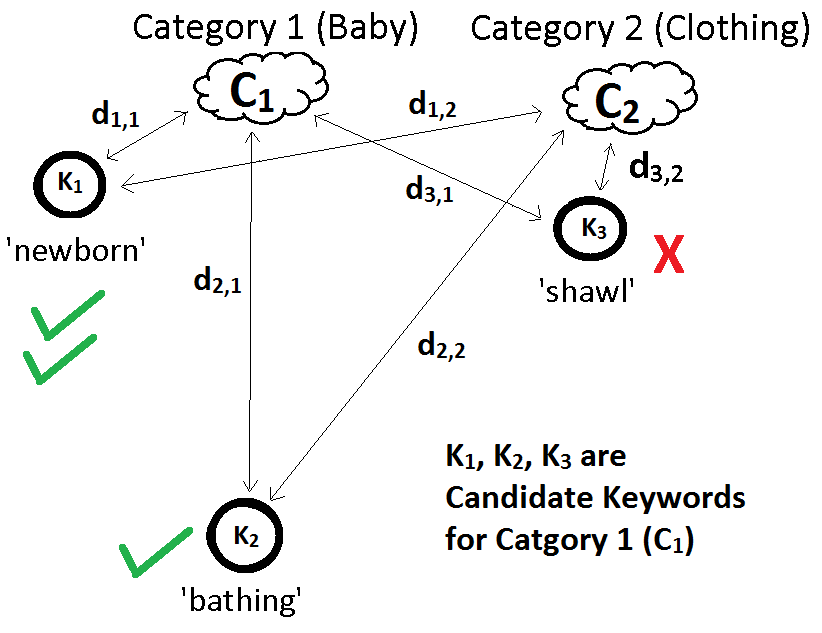
\includegraphics[width=0.6\linewidth]{TrainingData/WIfigures/keyword_properties_Baby2.png}
\caption{Selection criteria for Selected Retriever Keywords}
\label{fig:KeywordProperties}
\end{figure}

\label{sec:overviewselectSRK}
\begin{figure*}[htb!]
\centering
\begin{tabular}{cc}
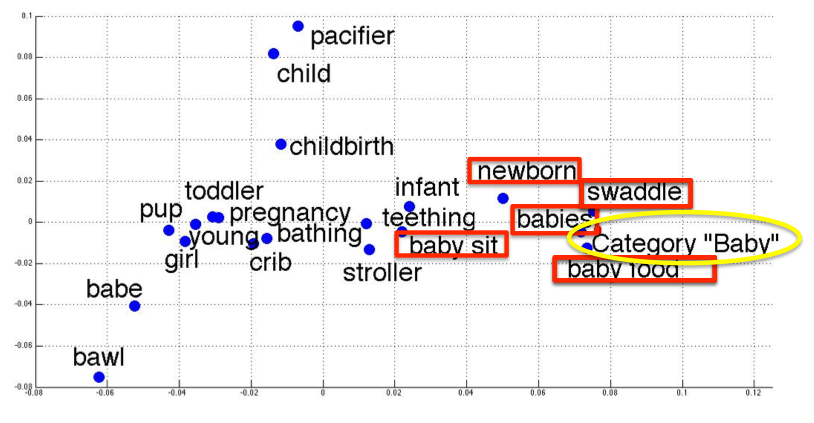
\includegraphics[width=0.47\textwidth,clip=]{TrainingData/figs/Baby_20_5_proxKwds.png} & 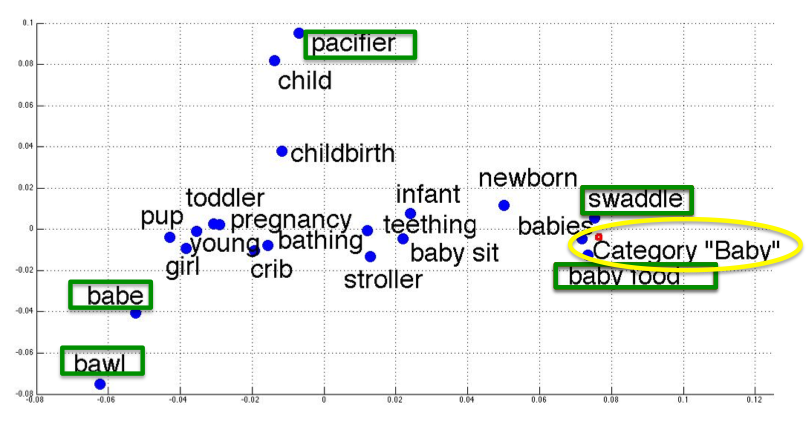
\includegraphics[width=0.47\textwidth,clip=]{TrainingData/figs/Baby_20_5_DiverseKwds.png}\\ 
(a) & (b) \\ 
\end{tabular}
\caption{\small{For a set of 20 valid keywords for the category `$Baby$', (a) shows the 5 most proximate keywords and (b) shows the 5 most diverse keywords. Diversity is measured as outlined in Section~\ref{sec:aao}. As can be seen, the set of keywords optimizing either objective function are very different from each other. Note that in order to plot the keywords on a graph, the first two dimensions obtained from principal component analysis (PCA)~\cite{jolliffe2002principal} are used. }}
\label{fig:proxdivkwdBabyExamplePCA}
\end{figure*}

Before we discuss suitability of candidates, and the selection procedure for SRKs, we provide the following result to help in our discussions. Consider the set of categories $\{i\}_{i=1}^{N_{Cat}}$, where each category $i$ is a multivariate normal distribution with mean $\mu_i$. Assume that the set of videos across all categories (referred to as data) is whitened, i.e., has uncorrelated dimensions of variance unity. Then $\Sigma_i = I$, i.e., the covariance matrices for all categories reduce to an identity matrix. Under assumptions of equiprobable categories, we derive that a video (represented as $v$) belongs to category $\hat{i}$ iff 
\begin{equation*} 
\hat{i}=\argmax_i{e^{-\frac{(v - \mu_i)^{T}\Sigma_i (v - \mu_i) }{2} }} \text{ , i.e., iff }
\end{equation*}
\begin{equation*} 
\hat{i}=\argmin_i{e^{ \mid v - \mu_i \mid ^{2}  }} \text{ , i.e., iff }
\end{equation*}
\begin{equation} \label{eq:proof6}
\hat{i}=\argmin_i{\mid v-\mu_i\mid}.
\end{equation}

Here $\mu_i$ is the mean of category $i$, as determined by an oracle. $ \mid v - \mu_i \mid$ is the Euclidean distance between $v$ and $\mu_i$. Note that for this paper, $v$ is represented as a bag of words~\cite{salton1975vector} vector based on the contextual information surrounding $v$. On the basis of the above assumptions, and using (\ref{eq:proof6}), a keyword $K$ retrieves more videos having true label as category $i$ than videos having true label as category $j ( \neq  i)$ if
\comment{
\begin{multline} \label{eq:proof7}
\sum_{v:v\in RV(K)}\mathcal{I}(\argmin_l{\mid v-\mu_l \mid}=i) \; \; \; > \\
\indent \sum_{v:v\in RV(K)}\mathcal{I}(\argmin_l{\mid v-\mu_l \mid}=j) \; \;  \forall j \neq i.
\end{multline}
}
\begin{equation}
\sum_{v:v\in RV(K)}\mathcal{I}(\argmin_l{\mid v-\mu_l \mid}=i) > \sum_{v:v\in RV(K)}\mathcal{I}(\argmin_l{\mid v-\mu_l \mid}=j)  \forall j \neq i.
\label{eq:proof7}
\end{equation}

Here, $\mathcal{I}(.)$ is an indicator function that is $1$ if its argument is true, and $0$ if its argument is false. $\mu_l$ is the true mean of category $l$. In (\ref{eq:proof7}), the closest category for each video in $RV(K)$ is obtained, in terms of Euclidean distance. Checking (\ref{eq:proof7}) for a keyword $K$ thus has complexity $O( \mid RV(K) \mid.N_{Cat})$, where $N_{Cat}$ is the number of categories, and $\mid RV(K) \mid$ is the cardinality of the set $RV(K)$. In order to reduce the above high complexity, (\ref{eq:proof7}) can be approximated by obtaining the closest category of centroid of the set $RV(K)$. This reduces the complexity to $O(N_{Cat})$. For category $i$, we define \textbf{Valid Candidate Keywords} (called valid keywords for brevity) as those Candidate Keywords that retrieve more videos having true label of category $i$ than of any other category. Then for a candidate $K$ of category $i$, $K$ is a valid keyword if 
\begin{equation} \label{eq:ValidityFilter}
\mid \mu_K - \mu_i \mid < \mid \mu_K - \mu_j \mid \forall j \neq i. 
\end{equation}
Here $\mu_K$ =  $\frac{ \sum{v:v \in RV(K)} }{\mid RV(K) \mid}$. The true mean $\mu_i$ for category $i$ can be approximated as centroid of $RV(C_i)$, i.e., of the set of videos retrieved by name of category $i$. Equation (\ref{eq:ValidityFilter}) is called the \textbf{Validity Filter}. Only valid keywords should be considered for being selected as SRK to ensure more number of training videos are added in $T(i)$ that have true label of category $i$ than videos that are mislabeled as category $i$. 

Note that we have assumed that the data generating the above distributions is whitened. If the given data is not whitened, its dimensions can be rotated into space of principal components, and each dimension divided by square root of variance in that dimension, in order to whiten the data. Also, if the assumption that categories are equiprobable multivariate normal distributions does not hold, then the exact distributions could be used to derive the Validity Filter as shown in (\ref{eq:ValidityFilter}). As a result, the complexity of checking the validity of a keyword may be more than $O(N_{Cat})$, however our approach of using a Validity Filter, and the following keyword selection procedure would still be valid. We continue our discussion with the above assumption. 

Let us consider the scenario shown in Fig.~\ref{fig:KeywordProperties}. Keywords $K_1$, $K_2$, $K_3$ are candidates for category $1$ ($C_1$). $K_3$, as can be seen, is closer in terms of Euclidean distance, to category $2$ ($C_2$) than to $C_1$, and hence fails the Validity Filter (\ref{eq:ValidityFilter}). For $C_1$ and $C_2$ as $Baby$ and $Clothing$ respectively, example keywords (from actual data) for $K_1$, $K_2$, $K_3$ are `$newborn$', `$bathing$',  `$shawl$' respectively. Note that a candidate may have a weak semantic relationship with its corresponding category name. For example, the candidates' source \cite{ReverseDictionary} recommends `$shawl$' as a candidate keyword for $Baby$ category since they are related perhaps owing to the use of shawls to cover or carry babies with. 
However querying `$shawl$' ($K_3$) in a video search engine is much less likely to retrieve $Baby$ related videos than it is to retrieve $Clothing$ related videos. Thus including $RV(`shawl\text{'})$ in training data of category $Baby$ would add more mislabeled videos in $T(Baby)$ than videos having true label of category $Baby$. Validity Filter (\ref{eq:ValidityFilter}) ensures that candidates such as `$shawl$' are not valid keywords for category $Baby$. 

Let $N_{Valid,i}$ be the number of valid keywords for category $i$. In order to select keywords form the valid keywords, we determine the suitability of keywords to retrieve training videos for category $i$ based on two components: 1) High Proximity, 2) High Diversity. We discuss below how the above components lead to training videos having the desired properties, less mislabeled videos and high Intra-Category Diversity respectively.  


\textbf{\textit{High Proximity.}} Under assumptions of whitened data and multivariate normal distributions as the categories, the likelihood of a video $v$ belonging to a category $i$ is proportional to $e^{(-\frac{1}{2}\mid v-\mu_i \mid^2)}$. Assuming equal prior probabilities for all categories, the probability that $v$ has its true label as category $i$ is higher when $\mid v - \mu_i \mid$ is lower, where $\mu_i$ is the true mean of category $i$. Thus, if $v$ is a video in training data of category $i$, then P(\textit{v is a mislabeled video}) is lower when $\mid v - \mu_i \mid$ is lower. Consider a valid keyword $K$ for category $i$. Satisfying (\ref{eq:ValidityFilter}) merely implies that $RV(K)$ contains more videos of true label category $i$ than videos that are mislabeled as category $i$. Preference should be given to valid keywords that lead to lesser mislabeled videos in the resulting set of training videos of category $i$. In order to do so, a valid keyword $K$ should be preferred if the videos in $RV(K)$ are closer to $\mu_i$. We thus calculate \textbf{Proximity score} for each valid keyword $K$ as 
\begin{equation} \label{eq:proximityscore}
\text{Proximity score for $K$}= \{ 1/\mid \mu_K - \mu_i \mid \}, 
\end{equation}
 where $\mu_K$ is the centroid of $RV(K)$. A keyword $K$ should be preferred to be selected as a Selected Retriever Keyword (SRK) if the Proximity Score of $K$ is high.  

In Fig.~\ref{fig:KeywordProperties}, `$newborn$' ($K_1$) and `$bathing$' ($K_2$) are both Valid Candidate Keywords for category $Baby$ ($C_1$). Since the centroid of $RV(\text{`}newborn\text{'})$ is closer to the mean of $C_1$ than the centroid of $RV(\text{`}bathing\text{'})$, the proximity score of `$newborn$' is more than that of `$bathing$'. Thus as per the proximity score, the valid keyword `$newborn$' should be preferred over `$bathing$'. Since \textit{P(true label of $v =C_1 \mid  v \in RV(\text{`}newborn\text{'})$)} is more than \textit{P(true label of $v =C_1 \mid  v \in RV(\text{`}bathing\text{'})$)}, preferring `$newborn$' over `$bathing$' as SRK reduces mislabeled videos in resulting set of training videos.  

Note that the measurement of Proximity score of a valid keyword is the same for both approaches proposed in Section~\ref{sec:overviewselectSRK}. 

\textbf{\textit{High Diversity.}} Intuitively, the diversity of a set of keywords reflects the Intra-Category Diversity of the set of videos that are retrieved using the keywords. For the LCPD approach discussed next in Section~\ref{sec:lcpd}, the Intra-Category Diversity of the training videos of category $i$, i.e., $div(T(i))$ is measured based on variance of the set of videos $T(i)$. Based on such a measure for $div(T(i))$, a diversity score can be defined for each keyword $K$ given a subset of the training data of category $i$, denoted by $T\text{'}(i)$. Details of such a \textit{per-keyword} measurement of Intra-Category Diversity are provided in Section~\ref{sec:lcpd}. As an alternative way, since training videos are retrieved using SRKs, the degree of variation in $T(i)$ could also be estimated based on the degree of variation in the set of keywords that are used to obtain them. Based on this insight, the second keyword selection approach (AAO approach in Section~\ref{sec:aao}) uses a diversity measure for a set of keywords, instead of a diversity measure per keyword as used in Section~\ref{sec:lcpd}. In order to obtain a diversity measure for a set of keywords, distance or linear independence based measures can be used. Section~\ref{sec:aao} discusses the efficiency implications of different diversity measures for set of keywords. For the AAO approach, we utilize linear independence based diversity measures for set of keywords. 

Based on the above discussion, SRKs need to be selected such that they have high proximity score, and high diversity. Selecting keywords based on high proximity tends to prefer keywords that retrieve videos similar or \textit{close} to those retrieved by the name of the category. On the other hand, selecting keywords based on high diversity tends to prefer keywords that are more different or \textit{far} from each other. Thus the two objectives tend to be opposing in nature. Figures~\ref{fig:proxdivkwdBabyExamplePCA}(a) and \ref{fig:proxdivkwdBabyExamplePCA}(b) provide an example of a set of 5 keywords selected based on either objective for a set of 20 valid keywords of the category `$Baby$'. As can be seen, the sets of keywords optimizing either objective are very different from each other and optimizing for one tends to lead to keywords having poor objective score for the other. In the next section, we propose approaches to address keyword selection problem based on such conflicting objectives. 


\section{Approaches to select SRKs}
\label{sec:selectionSRK}

In order to obtain SRKs from a set of valid keywords, we propose two efficient approaches. The first approach (LCPD) is based on defining a diversity score per keyword. By defining a linear combination of the proximity and diversity scores of keywords, we propose an iterative algorithm to select SRKs one by one. Such an approach leads to high accuracy in video classification based on varying a parameter that controls the relative importance given to the two objective functions, namely proximity score and diversity score of a selected keyword. However, since the best parameter value cannot be known beforehand, and is different for different sets of categories, we also propose an annealing based alternating optimization (AAO) approach. In the AAO approach, we utilize two iterative algorithms that optimize for either objective function and we combine them in a simulated annealing framework. In order to facilitate the second approach, we define diversity for a set of keywords. Such an approach doesn't need preferences to be embedded in form of parameters, however as compared to the first approach, it may suffer some performance loss. 


\subsection{Linear combination of proximity and diversity (LCPD) }
\label{sec:lcpd}

In this approach, we define Suitability for Retrieving Training video ($SRT$) score for a valid keyword $K$ as a score that indicates how suitable the valid keyword is to retrieve videos for category $i$ such that the resulting training data has the desired properties discussed in Section~\ref{sec:desiredpropdata}. $SRT$ score of a valid keyword is defined based on the Proximity score of the keyword as defined and measured in Section~\ref{sec:overviewselectSRK}, and the Diversity score as defined below. 

For the training data $T(i)$ of category $i$, the Intra Category Diversity $div(T(i))$ can be measured as the average pair-wise distance between the videos in $T(i)$, assuming a distance measure between the videos. The time-complexity of such a measure, however, is $O(N^2)$ where $N$ denotes the cardinality of $T(i)$. For the approach proposed in this section, we choose to estimate $div(T(i))$ by the variance of $T(i)$, primarily because of its low time-complexity $O(N)$. 

\begin{equation} \label{eq:diversityeqn}
\indent div(T(i)) =   \sqrt{\frac{\sum\limits_{j=1}^N \mid v_j - \mu_i \mid ^2}{N}}  , 
\end{equation}
where $\mu_i=\frac{\sum\limits_{j=1}^{N} v_j}{N}$; $v_j$ is a training video for category $i$, and $N$ is the cardinality of the set T($i$), i.e., $\left \{ v_j \in T(i) \right \}_{j=1}^{N}$.

%From the discussion in Section II, a valid keyword $K$ should be preferred if it leads to higher Intra-Category Diversity of the resulting set of training videos. 
Assume that $T\text{'}(i)$ is the current training data of category $i$, then the set of training videos of category $i$ when $RV(K)$ are added to $T\text{'}(i)$ would be  $\{T\text{'}(i) \cup RV(K)\}$. We hence define \textbf{Diversity score} of a valid keyword $K$ for category $i$, given existing training data $T\text{'}(i)$, as 
\begin{equation} \label{eq:divscorelcpd}
\text{Diversity score for $K$ given $T\text{'}(i)$} = div(T\text{'}(i) \cup RV(K)),
\end{equation}
where $div()$ can be calculated using (\ref{eq:diversityeqn}). 

For the set of categories {$Baby$, $Clothing$, $Fitness$, $Food$}, Table I shows the Proximity and Diversity scores for certain valid keywords of category $Baby$. For the purpose of calculation of these scores, the existing training data $T\text{'}(i)$ for category $i$ is taken to be $RV(C_i)$. The valid keyword `\textit{baby carriage}' has a high Proximity score, indicating it retrieves videos that are very close (in terms of Euclidean distance) to $RV(\text{`}Baby\text{'})$, but has a low Diversity score, indicating low Intra-Category Diversity of the resulting training data \{$RV($`\textit{Baby}'$) \cup RV($`\textit{Baby Carriage}'$)$\}. Compared to this, `$alert$' is a Valid Candidate Keyword for $Baby$ which has a high Diversity score, but has a very low Proximity score and hence very unlikely to retrieve Baby-related training videos.  Note that Table I only shows valid keywords so candidate keywords such as `$shawl$' that fail the Validity Filter are not provided.

\begin{table}
\fontsize{8pt}{1em}\selectfont
\begin{center}
\caption{{Proximity and diversity scores for a few valid keywords of category $Baby$, calculated as detailed in Section~\ref{sec:lcpd}}
\label{tab:PopularKeywords}}
\begin{tabular}{|c|c|c|}
		\hline
		\textbf{Valid Candidate Keyword} & \textbf{Proximity Score} & \textbf{Diversity score} \\
		\hline
		alert   & 0.607 & 0.3737\\
		\hline
		baby carriage & 3.346  & 0.2525\\
		\hline
		baby sit   & 2.815 & 0.2559\\
		\hline
		bassinet  & 3.148 & 0.3127\\
		\hline
		newborn  & 1.794 & 0.3495\\
		\hline
		swaddle  & 3.287 & 0.1899\\
		\hline
		tootsy  & 0.989 & 0.4769\\
		\hline
		bathing  & 0.756 & 0.2036\\
		\hline		
\end{tabular}
\vspace{-0.25in}
\end{center}
\end{table}

In order to combine the Proximity and Diversity scores to obtain $SRT$ score of a valid keyword $K$, we assume $SRT$ to be a simplistic linear combination of the two scores. $SRT(K, T\text{'}(i))$ denotes the Suitability for Retrieving Training video score of a valid keyword $K$  for category $i$, given that existing training data for category $i$ is $T\text{'}(i)$.  

$SRT(K, T\text{'}(i)) = $
\begin{equation} \label{eq:SRTeq}
\alpha * \left\{ \frac{N_1}{\mid \mu_K - \mu_i \mid}  \right\}  + (1-\alpha)*\left\{ N_2.div(T(i) \bigcup RV(K)     )  \right\}. 
\end{equation}

Here, $N_1$ and $N_2$ are normalization factors used to ensure that Proximity and Diversity scores have the same order of magnitude in (\ref{eq:SRTeq}). $\alpha \in \lbrack 0, 1 \rbrack$ is the \textbf{moderation factor}, which decides the weight given to the Proximity score relative to the Diversity score. We next discuss an iterative algorithm to obtain (a maximum of) $L$ keywords as SRK from a given set of candidates for each category, using $SRT$ as calculated in (\ref{eq:SRTeq}). 

\subsubsection{SRK Selection Algorithm for LCPD}
\label{sec:lcpdalgo}

The category names $C_i$, and number of SRKs to be selected ($L$) are inputs to the proposed SRK Selection Algorithm (Algorithm \ref{SRTAlgorithm}) shown below. Assume that $M$ Candidate Keywords are available for each category. Let the set of Candidate Keywords for category $i$ be $K_{Candidates,i}$. For each category, a set of valid keywords $K_{Valid,i}$ is selected as a subset of $K_{Candidates,i}$ that satisfy (\ref{eq:ValidityFilter}). Starting with $T\text{'}(i)=RV(C_i)$, $SRT(K, T\text{'}(i))$ is calculated for each valid keyword using (\ref{eq:SRTeq}), and the top keyword $K_{top}$ is selected as an SRK. $T\text{'}(i)$ is then updated to {$T\text{'}(i)  \cup RV(K_{top})$}, and the process is repeated until $L$ SRKs are selected or there are no valid keywords left. The proposed algorithm selects SRKs in an iterative manner, as compared to ranking valid keywords by their $SRT$ score calculated once and selecting the top $L$ keywords. While the latter calculates $SRT$ scores independent of other SRKs selected, the proposed algorithm attempts to increase Intra-Category Diversity of the resulting training data, leading to better performance of trained classification model.

For each category, number of valid keywords may be different and hence, the number of selected SRKs by the proposed algorithm need not be similar across different categories. In order to avoid any class imbalance, we select the first $L\text{'}$ SRKs for each category to obtain training videos, where $L\text{'}$ is the minimum number of SRKs selected by the proposed algorithm across all categories. $L\text{'} \le  L$ since a category may have less than $L$ valid keywords. The training videos retrieved by SRKs as per (\ref{eq:trainingDataUnioneqn}) can be utilized to train a classification model by giving equal weight or unequal weights to training videos, as discussed below. 
\begin{itemize}
\item \textbf{Non-Weighted Instances:} Classification model is trained by giving equal weight to all training instances (videos). 
\item \textbf{Weighted Instances:} Classification model is trained by giving a weight to a training video $v$ depending on the order in which the proposed algorithm selected the SRK corresponding to $v$. Consider a SRK $K$ that is selected for category $i$ by the proposed algorithm in the $n^{th}$ iteration. Each video $v$ in $RV(K)$ gets weight equal to ($1-1/n$). 
\end{itemize}
\begin{algorithm}
\fontsize{8pt}{1em}\selectfont
\caption{SRK selection algorithm for LCPD approach}
\label{SRTAlgorithm}
%\begin{algorithmic}[1]
\textbf{Inputs:} \\ 
\hspace*{2mm} Names of categories: $C_i$ \\
\hspace*{2mm} Number of SRKs: $L$ \\
\hspace*{2mm} Candidate keywords per category: $K_{Candidates, i}$\\
\hspace*{2mm}   (Note that the algorithm is run for each category) \\ 
%\Procedure{ArraySum}{$A$}
\textbf{Initialization:} \\ 
\hspace*{2mm} $K_{SRK, i} \leftarrow  [ \ ] \text{~(empty set)}$ \\
\hspace*{2mm} $T\text{'}(i) \leftarrow  RV(C_i)$ \\
\textbf{Applying Validity Filter:} \\
\hspace*{2mm} $K_{Valid,i} \leftarrow \{K \in K_{Candidates, i} \}: K$ satisfies (\ref{eq:ValidityFilter}) \\
\textbf{Iterative Algorithm:} \\
%\begin{tabbing}
\hspace*{2mm} For $n$=1 to $L$ (each iteration) \\
%\hspace*{6mm} For $i$=$1$ to $N_{Cat}$ (each cattegory) \\
\hspace*{6mm}  If $\mid K_{Valid, i}\mid=0$: STOP \\ 
\hspace*{6mm}  Calculate $SRT(K,T\text{'}(i)) \forall K \in K_{Valid, i}$ as per (\ref{eq:SRTeq})  \\
\hspace*{6mm}  \text{$K_{top}  \leftarrow \argmax_K{SRT(K,T\text{'}(i))}$} \\
\hspace*{6mm}  $K_{SRK, i} \leftarrow K_{SRK, i} \cup K_{top}$ \\ 
\hspace*{6mm}  $T\text{'}(i) \leftarrow  T\text{'}(i) \cup RV(K_{top})$ \\
\hspace*{6mm}  $K_{Valid, i} \leftarrow K_{Valid, i} \setminus K_{top}$ \\
%\hspace*{6mm} EndFor\\
\hspace*{2mm} EndFor \\ 
\textbf{Output:} $K_{SRK, i}$
%\end{tabbing}
%    \State $sum = 0$
%    \For {each integer $i$ in $A$}
%        \State $sum = sum + i$
%	\EndFor
%	\State Return $sum$
%\EndProcedure
%\end{algorithmic}
\end{algorithm}

\textbf{Analysis of Algorithm~\ref{SRTAlgorithm} and proposed methods.}
For the two methods described above, if the candidates are distinct, selecting more SRKs is in general expected to increase the Intra-Category Diversity, thus leading to better performance. However, after certain number of SRKs are selected, it is expected that the additional information of the new topics coming into the training data will reduce, and performance might saturate. Also, the SRKs selected in earlier iterations were determined to be more suitable for retrieving training videos than ones selected later by Algorithm~\ref{SRTAlgorithm}. The SRKs selected in last few iterations might not be very suitable to retrieve training videos of the respective category although they cleared the Validity Filter. Such SRKs might add videos of topics beyond the realm of categories of interest, and make the training data too general and less discriminative. Hence, the performance of Non-Weighted Instances method might peak at a certain $L$, and then degrade since it gives equal weight to training videos retrieved by all SRKs. In the Weighted Instances method however, the weight given to videos retrieved by SRKs accepted later is lesser. This makes the trained classifier less influenced by videos retrieved by SRKs that are selected in the last few iterations by the Algorithm~\ref{SRTAlgorithm}. Thus, unlike in the case of the Non-Weighted Instances method, the performance of Weighted Instances method may saturate with increasing $L$. The number of SRKs that lead to best classification performance for Non-Weighted Instances method may vary with the set of categories, the number and source of candidate keywords, among other factors. It is hence a better approach to choose as large $L$ as permitted by computational resources, and utilize the training videos for training of classification model, using the Weighted Instances method.

\textbf{Complexity analysis for Algorithm~\ref{SRTAlgorithm}.}
The time-complexity of Algorithm~\ref{SRTAlgorithm} is $O(M.N_{Cat}.L)$,  where $M$  is the number of candidates for each category, $N_{Cat}$ is number of categories, and $L$ is the number of SRKs selected. This is because in every iteration, the valid keywords for each category are given an $SRT$ score, and the maximum number of iterations that the proposed algorithm can run for is $L$. For fixed $M$ and $N_{Cat}$, the time-complexity of proposed algorithm varies as $O(L)$. The space-complexity of the proposed algorithm is $O(L)$ when the number of videos retrieved per SRK is kept constant. For learning tasks, when a very large sized training data is available, the size of training data used for training a model is generally constrained based on space and time-complexity of the employed learning algorithms, and available resources. Such constraints can dictate the total number of SRKs, i.e., $L$, utilized to retrieve training videos. In the following section, we provide observed space requirement, and time taken by the proposed algorithm based on our implementation, as well as its performance. 

The moderation factor $\alpha$ controls the relative importance given to proximity and diversity scores of valid keywords, and thus controls the set of SRKs that are finally selected. The value of $\alpha$ that leads to best performance of the video classification model depends on the category in concern, and on its set of candidate keywords and is thus hard to estimate beforehand. As will be shown in Section~\ref{sec:expt}, the video classification accuracy varies substantially with the moderation factor $\alpha$. Thus, as is also discussed in Section~\ref{sec:intro}, a shortcoming of the LCPD approach is that it requires a pre-determined value for the moderation factor $\alpha$, which may not be always available. So we next propose an approach that balances the objective functions of proximity and diversity of a set of keywords in a simulated annealing framework, thus converging to a unique solution, without the need to articulate preferences or bias towards either objective apriori.  
\subsection{Annealing based alternating optimization (AAO) for proximity and diversity maximization}
\label{sec:aao}
In this section, we describe an approach where two iterative algorithms, each optimizing for a certain objective function, are run alternately in order to obtain a solution that is a mutual trade-off between the two objectives. The two algorithms have the task of selecting a set of $L$ keywords amongst the valid keywords, such that the selected set maximizes average proximity and diversity respectively. The algorithms are discussed in detail in Sections~\ref{sec:aaoproxmax} and \ref{sec:aaodivmax} respectively. The methodology adopted for measuring average proximity and diversity of the set of selected keywords for the purpose of this approach is described next.  

\subsubsection{Measurement of proximity and diversity scores}
\label{sec:proxdivmeasureAAO}

For the AAO approach, proximity of a keyword $K$ is measured as detailed in Section~\ref{sec:overviewselectSRK}. For the LCPD approach, diversity was measured as the variance of the set of videos retrieved. Based on this, a diversity score per keyword given a training data was defined (\ref{eq:divscorelcpd}). Such a measurement was feasible for LCPD as it does not need to employ an algorithm to maximize the diversity of a set of keywords. In contrast to LCPD, the AAO approach measures diversity for a set of keywords, and not per keyword given certain training data. Using such a diversity measure, AAO employs an efficient algorithm capable of selecting the set of $L$ keywords that has the maximum diversity. In order to define diversity for a set of keywords, we first represent each keyword $K$ by the centroid of its retrieved videos $RV(K)$. The diversity of a set of keywords could be defined based on certain pair-wise distances measures between the keywords, however an optimization technique based on such a measure would essentially boil down to performing a combinatorial search over all $L$-sized subsets of the set of valid keywords, making it highly inefficient if not infeasible. As an example, for selecting 25 keywords from 200 valid keywords, this means going through ${200 \choose 25}$ i.e., around $4*10^{31}$ subsets. Hence, for AAO we develop a different way of measuring diversity: the diversity of a set of keywords is defined based on the degree of linear independence between the keywords. Doing so leads to highly efficient optimization through Rank-Revealing QR (RR-QR) factorizations, to obtain which efficient algorithms have been proposed in literature \cite{BusingerLinear65,GolubNumeri65,ChanRank87,GuEfficient96}. 

Assume that the set of $L$ keywords for which we would like to calculate the diversity is $x_L = \{K_j\}$ where $j$ = $1$ to $L$. The matrix representation of $x_L$ is $X_L \in \mathbb{R} ^{m\times L} $ where $m$ is the dimensionality of the representation of each video i.e., the size of the bag of words representation of each video, and $m \ge L$. The $j^{th}$ column of $X_L$ is represented as $\mu_{Kj}$ i.e., as the centroid of the set of videos RV($K_j$). The \textbf{diversity score} of the set of keywords $x_L$ is then defined as 
\begin{equation} \label{eq:divaao}
\text{Diversity score for $x_L$}=\prod_{b}{\sigma_b(X_L) }, 
\end{equation}
 where $\sigma_b(X_L)$ is the $b^{th}$ singular value of the matrix $X_L$. 

\subsubsection{Overall Approach for AAO}
\label{sec:overallAAO}

The AAO approach optimizes for two objectives (average proximity score, and diversity score of a set of keywords) alternately, under a simulated annealing framework. Average proximity score of a set of keywords, as the name implies, is the average of the proximity scores of the keywords in the set. This is represented as $O_{Proximity}$. Diversity score of a set of keywords is represented as $O_{Diversity}$ and is calculated using~(\ref{eq:divaao}). The two iterative algorithms that optimize for these objective functions individually can converge to the most proximate or the most diverse set of keywords respectively. However, we add a constraint parameter $T$ where $T \in \lbrack 1, \infty)$ in the framework that controls the extent to which each algorithm is permitted to run. The individual optimization algorithms are such that $T$ can be provided as an input. They also take a set of keywords as input for the initial solution and improve the solution in each iteration. For a lenient (lower) value of $T$, either of the algorithms is permitted to run for more number of iterations and as a result, the solution at the end of the run is better in terms of the corresponding objective function. The constraint parameter $T$ is set to $1$ to start with, which allows both algorithms to optimize for their respective objective functions. 

\begin{figure}
\centering
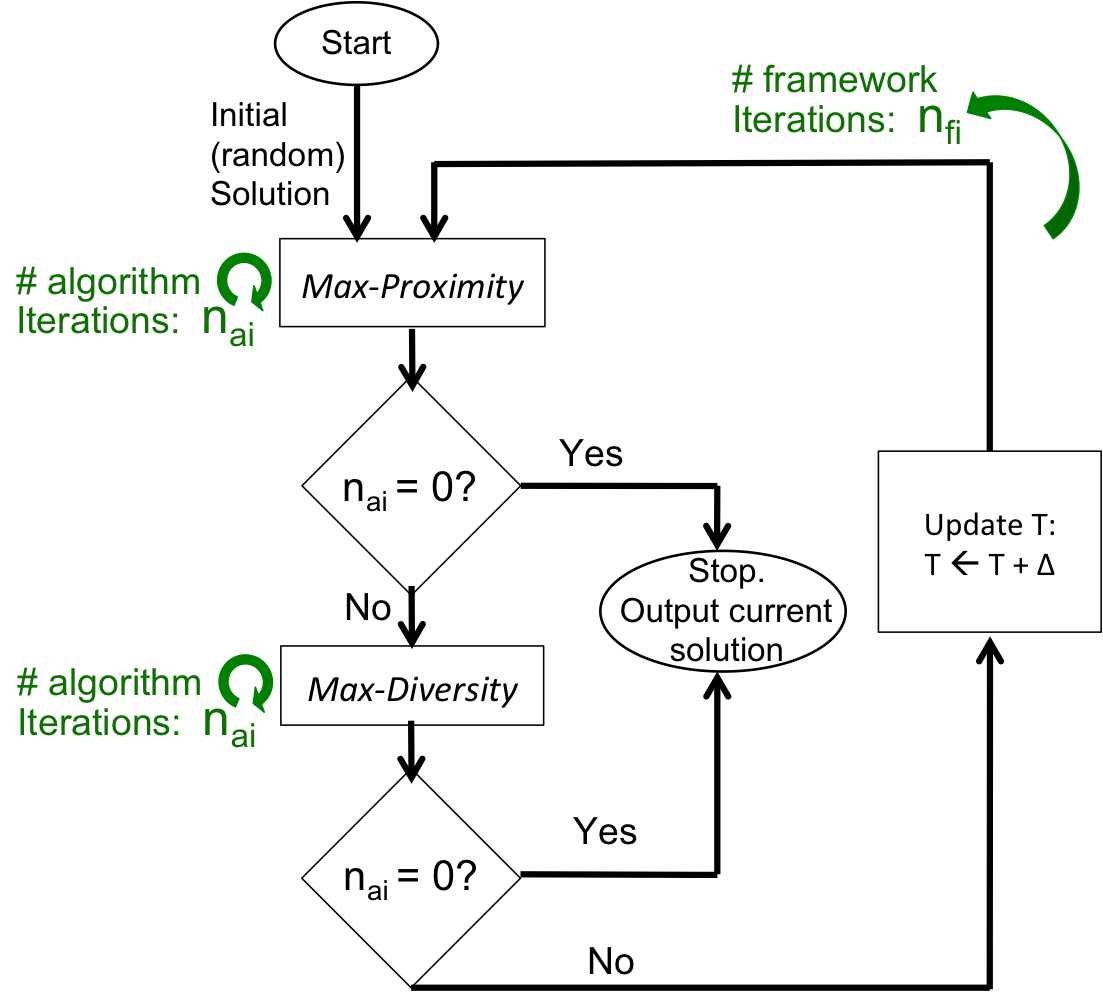
\includegraphics[width=0.75\linewidth]{TrainingData/figs/aao_overview.png}
\caption{Overview of the AAO approach for alternately optimizing the average proximity and diversity of selected keywords}
\label{fig:AAOoverview}
\end{figure}

Fig.~\ref{fig:AAOoverview} gives an overview of the AAO approach. The iterative algorithm to optimize for $O_{Proximity}$ (shown as \textit{Max-Proximity} in Fig.~\ref{fig:AAOoverview}) is initially run based on a random set of $L$ keywords and $T=1$, and selects the set of $L$ keywords that has the highest average proximity. This set is provided as input to the iterative algorithm to optimize for $O_{Diversity}$ (shown as \textit{Max-Diversity} in Fig.~\ref{fig:AAOoverview}), along with the same value of $T$. This leads to the selection of a set of $L$ keywords having the maximum diversity score. This completes the first iteration of the AAO framework, also referred to as the first \textbf{framework iteration}. Framework iterations are represented by $n_{fi}$. For 20 valid candidate keywords of the category Baby and for $T=1$, the sets of 5 keywords obtained at the end of either algorithm are provided in Figures~\ref{fig:proxdivkwdBabyExamplePCA}(a) and \ref{fig:proxdivkwdBabyExamplePCA}(b) respectively. The output, i.e., the set of keywords selected at the end of the first framework iteration is then routed back to the \textit{Max-Proximity} algorithm to start the second framework iteration. At this point, the constraint parameter $T$ is increased by a constant amount $\Delta$ to a higher and thus a stricter value. As a result of the stricter value of $T$, the algorithm \textit{Max-Proximity} is constrained from running completely. While it may select a set of keywords with higher average proximity than the output of first framework iteration, the set of keywords selected may not maximize the average proximity as the algorithm was prevented from running completely. This process continues and the value of $T$ is increased at the end of each framework iteration, thus making it harder for the algorithms to select keywords that maximize their corresponding objective functions. The framework stops when either of the two algorithms cannot proceed. 

The sets of selected keywords obtained at the end of the algorithms \textit{Max-Proximity} and \textit{Max-Diversity} vary a lot with each other in the initial framework iterations. This can be seen in Fig.~\ref{fig:proxdivVariationAAO}(b) where a higher intensity of colors (red or blue) reflects a higher value of the corresponding objective function (average proximity or diversity respectively). As $T$ increases, the variation in the outputs at the end of the two algorithms reduces. The overall annealing based optimization framework is detailed in Algorithm II. Note that the overall framework is iterative and the individual algorithms that maximize average proximity or diversity are iterative too. In order to avoid confusion, an iteration of either \textit{Max-Proximity} algorithm, or of \textit{Max-Diversity} algorithm is referred to as an \textbf{algorithm iteration} and is represented by $n_{ai}$. Details on the individual iterative algorithms that optimize for the two objective functions are provided in the next section. Note that the proof of convergence for Algorithm II is given after describing \textit{Max-Proximity} and \textit{Max-Diversity} algorithms since the proof requires convergence properties of \textit{Max-Proximity}. 

In Section~\ref{sec:adaptAAO} we study the effect of $\Delta$ on the convergence of the AAO framework, specifically on the resulting set of keywords after convergence and on the time taken to converge. Further, in order to reduce the time taken by the optimization framework to converge without inducing bias in the end result, we propose an adaptive technique to update the constraint parameter $T$ based on the \textit{weakest permitted} algorithm iteration of the previous framework iteration. Details and the definition of the weakest permitted algorithm iteration are provided in Section~\ref{sec:adaptAAO}. 

\begin{algorithm}
\fontsize{8pt}{1em}\selectfont
\caption{Annealing based alternating optimization (AAO) framework for maximizing average proximity and diversity of selected keywords}
\label{algo:AAO}
\textbf{Inputs:} \\ 
\hspace*{2mm}          Number of keywords: $L$ \\ 
\hspace*{2mm}          Set of valid keywords: $K_{Valid}$ \\
\hspace*{2mm}          Representation of valid keywords in matrix form: $X$ \\
\hspace*{2mm}          Proximity score $\forall K \in K_{Valid}$ \\
\hspace*{2mm}          Increment for constraint parameter ($T$): $\Delta$ \\ 	
\hspace*{2mm}   (Note that the subscript $i$ is dropped since the algorithm is  \\ 
\hspace*{2mm}   run for each category separately) \\ 
\textbf{Initialization:} \\ 
\hspace*{2mm}       $K_{SRK}$ $\leftarrow$ set of random $L$ keywords from $K_{Valid}$\\ 
\hspace*{2mm}          $T \leftarrow 1$ \\ 
\hspace*{2mm}          $n_{fi} \leftarrow 0$  \\ 
\textbf{Begin framework iterations: } \\ 
\hspace*{2mm}       While (1) 		 \\ 
\hspace*{6mm}        \textbf{Maximize proximity:} \\ 
\hspace*{6mm}        ($K_{SRK}$, $n_{ai}$) $\leftarrow$ \textit{Max-Proximity}($K_{SRK}$, $T$, Proximity scores) \,\,\,\,\,\,\,\,\,\,\,\,\,\,\,\,\,\,\,\,\,\,\,\,\,\\
\hspace*{6mm}        If ($n_{ai} = 0$):  STOP \\
\hspace*{6mm}        \textbf{Maximize diversity: } \\ 
\hspace*{6mm}        ($K_{SRK}$, $n_{ai}$) $\leftarrow$ \textit{Max-Diversity}($K_{SRK}$, $T$, $X$) \\
\hspace*{6mm}        If ($n_{ai} = 0$):  STOP    \\ 
\hspace*{6mm}        $T \leftarrow T + \Delta$ (increment constraint parameter) \\ 
\hspace*{6mm}        $n_{fi} \leftarrow n_{fi} + 1 $ \\ 
\hspace*{2mm}       End While \\ 
\textbf{Output:} Selected set of retriever keywords: $K_{SRK} $  
\end{algorithm}




\begin{algorithm}
\fontsize{8pt}{1em}\selectfont
\caption{Max-Proximity algorithm}
\label{algo:maxproximity}
\textbf{Inputs:}  \\ 
\hspace*{2mm}   Initial set of selected keywords: $I_{SRK}$ \\ 
\hspace*{2mm}   Constraint parameter: $T$ \\ 
\hspace*{2mm}   Valid keywords $K_{Valid}$ and Proximity score $\forall K \in  K_{Valid}$ \\ %  as Proximity($K$)  \\ 
\hspace*{2mm}   (Note that the subscript $i$ is dropped since the algorithm is \\ 
\hspace*{2mm}   run for each category separately) \\ 
\textbf{Initialization:} \\ 
\hspace*{2mm}  $L \leftarrow \mid I_{SRK} \mid$ \\ 
\hspace*{2mm}   $K_{SRK} \leftarrow I_{SRK} $ \\   
\hspace*{2mm}   $WI_{Proximity} \leftarrow$ an arbitrarily large value \\ 
\hspace*{2mm}   ($WI_{Proximity}$: Weakest permitted algorithm iteration) \\ 
\hspace*{2mm}   $n_{ai} \leftarrow 0$ \\ 
\textbf{Begin framework iterations: } \\ 
\hspace*{2mm} While (1) 		 \\ 
\hspace*{6mm}        $O_{Proximity} \leftarrow $ Average proximity score of $K_{SRK}$ \\       
\hspace*{6mm}               Replace least proximate keyword in $K_{SRK}$ with most proximate keyword in \{$K_{Valid} \setminus K_{SRK}$\} to get $K\text{'}_{SRK}$  \\ 
\hspace*{6mm}               $O\text{'}_{Proximity} \leftarrow$ Average proximity score of $K\text{'}_{SRK}$ \\  
\hspace*{6mm}               If $\frac{O\text{'}_{Proximity}}{O_{Proximity}} > T$: \\ 
\hspace*{10mm}               $K_{SRK} \leftarrow K\text{'}_{SRK}$ \\ 
\hspace*{10mm}                           If $\frac{O\text{'}_{Proximity}}{O_{Proximity}}  < WI_{Proximity}$:\\ 
\hspace*{14mm}        	         $WI_{Proximity} \leftarrow \frac{O\text{'}_{Proximity}}{O_{Proximity}} $ \\ 
\hspace*{6mm}               Else:  STOP \\  
\hspace*{6mm}        $n_{ai} \leftarrow n_{ai} + 1 $ \\ 
\hspace*{2mm} End While \\ 
\textbf{Outputs: } \\ 
\hspace*{2mm}Selected set of retriever keywords: $K_{SRK}$ \\ 
\hspace*{2mm}$WI_{Proximity}$ (useful for Algorithm \ref{algo:AdaptAAO}) \\
\hspace*{2mm}Number of algorithm iterations: $n_{ai}$
\end{algorithm}

\subsubsection{Average proximity score maximization }
\label{sec:aaoproxmax}

The proximity scores of valid keywords for a category are fixed values defined as per (\ref{eq:proximityscore}). The easiest way to maximize the average proximity of selected $L$ keywords from the set of valid keywords for category $i$, i.e., from $K_{Valid,i}$, is to select the $L$ keywords from $K_{Valid, i}$ having the highest proximity scores. However such an approach does not permit adding a constraint parameter ($T$) to control the extent to which the proximity maximization algorithm is run. In order to do that, we propose an iterative algorithm \textit{Max-Proximity} that maximizes the average proximity of selected $L$ keywords by performing exchanges or swaps between the selected keywords and the non-selected valid keywords. \textit{Max-Proximity} is presented in Algorithm~\ref{algo:maxproximity}. Each iteration of the algorithm checks if replacing the selected keyword having the least proximity score (i.e., the least proximate selected keyword) with the most proximate non-selected valid keyword leads to a \textit{relative benefit} in average proximity above the constraint parameter $T$. The relative benefit is defined as a ratio of the average proximity of the selected keywords after the swap, with the average proximity before the swap. If that is the case, the above mentioned two keywords are swapped and the set of selected keywords $K_{SRK,i}$ is updated. If not, the algorithm terminates since this means no other swap between the keywords would lead to a relative benefit in average proximity above $T$. The algorithm takes as input and starts from a set of $L$ keywords as $K_{SRK,i}$, referred to in Algorithm~\ref{algo:maxproximity} as $I$. When $T$ is equal to $1$, any improvement in the average proximity score is acceptable and \textit{Max-Proximity} converges to the set of $L$ keywords having highest proximity scores. 

\textbf{Proof of correctness for Algorithm~\ref{algo:maxproximity}. } 
%\begin{proof}
We prove that \textit{Max-Proximity} (Algorithm~\ref{algo:maxproximity}) leads to maximization of the average proximity score when permitted to run completely, i.e., when $T=1$. Assume that $S_{OptProx}$ is the optimal set of keywords that maximizes the average proximity score amongst a set of valid keywords $K_{Valid}$. $S_{OptProx}$ then comprises of the $L$ keywords in $K_{Valid}$ which have the highest proximity score. Also assume that $S_{init}$ is the set of valid keywords that are given as initialization to Algorithm~\ref{algo:maxproximity}. The cardinality of $S_{init}$ is $L$, the number of keywords that are to be selected by \textit{Max-Proximity}. Then, there are ($\mid S_{OptProx} \cap S_{init} \mid$) keywords in $S_{init}$ that are also in $S_{OptProx}$, and are also the ($\mid S_{OptProx} \cap S_{init} \mid$) most proximate keywords in $S_{init}$. In $\mid S_{OptProx} \setminus S_{init}  \mid$ iterations of Algorithm~\ref{algo:maxproximity}, the  $\mid S_{OptProx} \setminus S_{init} \mid$ least proximate keywords from $S_{init}$ will be exchanged (swapped) with the keywords in the set $S_{OptProx} \setminus S_{init}$ in the order of decreasing proximity score of the latter. All such exchanges replace a keyword having a lower proximity score with another having a higher proximity score. Thus, the average proximity score of the selected keywords goes up by some amount in each iteration and since $T=1$, any improvement would be acceptable. Thus, at the end of $\mid S_{OptProx} \setminus S_{init} \mid$ iterations, the set of keywords that will be selected will be $S_{OptProx}$. \hfill $\square$
%\end{proof}

As a corollary, since \textit{Max-Proximity} takes $\mid S_{OptProx} \setminus S_{init} \mid$ iterations to select the set of most proximate keywords, and since  $\mid S_{OptProx} \setminus S_{init} \mid$ can take a maximum value of $L$, the maximum number of iterations that \textit{Max-Proximity} can run for is $L$. 

\textbf{Complexity analysis for Algorithm~\ref{algo:maxproximity}.} The complexity of Algorithm~\ref{algo:maxproximity} per keyword exchange is $O(L (N_{Valid} -L))$ where $L$ is the number of SRKs. Since $N_{Valid} \ge L$, and the maximum number of algorithm iterations is $L$, the worst case complexity of Algorithm~\ref{algo:maxproximity} is $O(L^2 N_{Valid})$. 


\subsubsection{Diversity score maximization}
\label{sec:aaodivmax}
\begin{algorithm}
\fontsize{8pt}{1em}\selectfont
\caption{Max-Diversity algorithm }
\label{algo:maxdiversity}
\textbf{Inputs:}  \\ 
\hspace*{2mm}   Initial set of selected keywords: $I_{SRK}$ \\ 
\hspace*{2mm}   Constraint parameter: $T$ \\ 
\hspace*{2mm}   Valid keywords $K_{Valid}$ and their matrix form: $X$ \\ 
%\hspace*{2mm}    corresponding to the set $K_{Valid}$ \\ 
\hspace*{2mm}   (Note that the subscript $i$ is dropped since the algorithm is  \\ 
\hspace*{2mm}   run for each category separately) \\ 
\textbf{Initialization:} \\ 
\hspace*{2mm}   $L \leftarrow \mid I_{SRK} \mid$ \\ 
\hspace*{2mm}   $K_{SRK} \leftarrow I_{SRK} $ \\   
\hspace*{2mm}   Obtain $\Pi_{init}$ such that keywords in $K_{SRK}$ are the \\
\hspace*{2mm}   first $L$ columns of $X$ \\ 
\hspace*{2mm}   $X \leftarrow X \Pi_{init} $ (rearrange columns of $X$)  \\ 
\hspace*{2mm}   $WI_{Diversity} \leftarrow $ an arbitrarily large value \\ 
\hspace*{2mm}   ($WI_{Diversity}$: Weakest permitted algorithm iteration) \\ 
\hspace*{2mm}   $n_{ai} \leftarrow 0$ \\ 
\textbf{Begin framework iterations: } \\ 
\hspace*{2mm}   While (1) 		 \\ 
\hspace*{6mm}        Compute QR factorization of X to get $A_L$, $B_L$, $C_L$ \\ 
\hspace*{6mm}        as per (\ref{eq:rrqr})  \\ 
\hspace*{6mm}        Calculate $G_{i,j}$ as: 
\begin{equation}
G_{i,j} = \sqrt{  ( A_L^{-1} B_L )^2 _{i,j}   + (\frac{\gamma_j(C_L)}{w_i(A_L)}  )^2 } 
\end{equation}

\hspace*{6mm}        Obtain the best swap as: $(\hat{i}, \hat{j}) \leftarrow \argmax_{i,j}{G_{i,j}}$ \\ 
\hspace*{6mm}        If $G_{\hat{i}, \hat{j}} > T$: \\ 
\hspace*{10mm}                           Update $K_{SRK}$: Replace $\hat{i}^{th}$ keyword of $K_{SRK}$ \\
\hspace*{10mm}                           with $\hat{j}^{th}$ keyword of $K_{Valid}  \setminus K_{SRK}$ \\ 
\hspace*{10mm}                           $X \leftarrow X \Pi_{ \hat{i} \leftrightarrow (\hat{j} + L) }$ \\ 
\hspace*{10mm}                           If $G_{ \hat{i}, \hat{j} }  < WI_{Diversity}$:  $WI_{Diversity} = G_{\hat{i}, \hat{j} }$ \\ 
\hspace*{6mm}               Else:  STOP \\ 
\hspace*{6mm}        $n_{ai} \leftarrow n_{ai} + 1 $ \\ 
\hspace*{2mm}   End While \\ 
\textbf{Outputs: }  \\ 
\hspace*{2mm}   Selected set of retriever keywords: $K_{SRK}$ \\ 
\hspace*{2mm}   $WI_{Diversity}$ (useful for Algorithm \ref{algo:AdaptAAO}) \\
\hspace*{2mm}   Number of algorithm iterations: $n_{ai}$
\end{algorithm}
We propose to use Rank Revealing QR factorization (RRQR) \cite{GuEfficient96} to select keywords having the highest diversity, where diversity of a set of keywords is measured using (\ref{eq:divaao}), since there exist efficient algorithms to provide RRQR factorization \cite{GuEfficient96,GolubNumeri65}. RRQR factorization has also been used in \cite{ShroffManifold11} to obtain diverse video frames for the application of video summarization. Let $x_i$ be the set of valid candidate keywords for category $i$. The discussion in this section is for a fixed category (category $i$) and so the subscript $i$ is dropped for convenience. Thus the set of valid keywords is represented as $X = \{K_j\}$ where $j$ = $1$ to $N_{Valid}$. As mentioned in Section~\ref{sec:proxdivmeasureAAO}, the matrix representation of $x$ is $X \in \mathbb{R}^{m\times N_{Valid}}$ where $m$ is the number of dimensions used to represent each valid keyword  and $m \ge N_{Valid}$. In order to describe the algorithm used to select the $L$ keywords from $x$ that maximize diversity, we first provide a brief discussion on RRQR factorization \cite{GuEfficient96,GolubNumeri65} and its objectives. 

Given a matrix $X \in \mathbb{R}^{a\times b}$ where $a \ge b$, consider the partial QR factorization of the form

\begin{equation} \label{eq:rrqr}
X \Pi = Q R = Q \bigl(\begin{smallmatrix}
A_L & B_L\\ 
 & C_L
\end{smallmatrix}\bigr),  
\end{equation}
where $Q \in \mathbb{R}^{a\times a}$ is an orthogonal matrix with nonnegative diagonal elements, $A_L \in \mathbb{R}^{L\times L}$ is an upper triangular matrix, $B_L \in \mathbb{R}^{L\times (b-L)}$ and $C_L \in \mathbb{R}^{(a-L)\times (b-L)}$. $\Pi \in \mathbb{R}^{b\times b}$ is a permutation matrix that is a square binary matrix having exactly one $1$ in each row and each column and $0$ everywhere else. $\Pi$ represents a specific permutation of the columns of the matrix $X$ and the permuted matrix can be obtained as $X \Pi$. For a given permutation $\Pi$, $X \Pi$ can be written as ($X_L$  $X_{(b-L)}$) where $X_L \in \mathbb{R}^{a\times L}$ is the matrix formed by the first $L$ columns of $X$, and $X_{(b-L)} \in \mathbb{R}^{a\times (b-L)}$ is the matrix formed by the last ($b-L$) columns of $X$. The degree of linear independence of the first $L$ columns of $X \Pi$ can be obtained as the determinant of the matrix $A_L$, also equal to the product of the singular values of the matrix $X_L$, i.e., $\prod_{j}{\sigma_j(X_L) }$. RRQR factorization aims to find the permutation $\Pi$ such that $X \Pi $ = ($X_L$  $X_{(b-L)}$) reveals the rank of the matrix $X$. This permutation $\Pi$ provides $X_L$ the $L$ most linearly independent columns of $X$. RRQR factorization does so by seeking $\Pi$ which maximizes the product of singular values of $X_L$. Please refer to \cite{BusingerLinear65,GolubNumeri65,ChanRank87,GuEfficient96} for further details and for proof of correctness of RRQR factorization. 

In order to adopt RRQR for AAO approach, we need to add a constraint on the RRQR algorithm based on the parameter $T$. Hence, in each algorithm iteration of RRQR, the \textit{relative benefit} is defined as the ratio of new and previous objective functions. The relative benefit is compared with $T$ to determine if the updated set of keywords is acceptable or not (Algorithm~\ref{algo:maxdiversity}). This ratio is represented as $G_{i,j}$ in Algorithm~\ref{algo:maxdiversity}. Since $T \ge 1$, this ensures that within a framework iteration of AAO, the diversity only increases with each algorithm iterations of RRQR algorithm. Note that in Algorithm~\ref{algo:maxdiversity}, for a non-singular matrix $W \in \mathbb{R}^{L\times L}$, $1/w_i(W)$ denotes the 2-norm of the $i^{th}$ row of $W^{-1}$. Also, for a matrix $W\text{'}$ with $L$ columns, $\gamma_j(W\text{'})$ denotes the 2-norm of the $j^{th}$ column of $W\text{'}$. 

\textbf{Complexity analysis for Algorithm~\ref{algo:maxdiversity}.} Using results from \cite{GuEfficient96}, the worst case time taken by Algorithm~\ref{algo:maxdiversity} is $O(mLN_{Valid})$ where $m$ is the number of dimensions used to represent each valid keyword. 

\textbf{Proof of convergence for Algorithm~\ref{algo:AAO}.}
Algorithm~\ref{algo:AAO} calls \textit{Max-Proximity} with an input set of $L$ keywords. We will first show that if the constraint parameter $T$ is increased beyond a value, $T_{MaxGainProx}$, then no iteration of \textit{Max-Proximity} can take place. Let $K_{LowP}$ and $K_{HighP}$ be distinct valid keywords with lowest and highest proximity score respectively. Let $S$' represent certain set of $L-1$ distinct valid keywords, and let $S$ represent the set of selected keywords in an iteration of \textit{Max-Proximity}, such that $S = S\text{'} \cup K_{LowP}$ and $K_{HighP} \not\in S$. The maximum relative gain in the average proximity score of selected keywords by exchanging one keyword would be when $K_{LowP}$ is replaced with $K_{HighP}$. Thus, the maximum relative change in the average proximity score of selected keywords can be $\frac{ Pr(K_{HighP}) + Pr(S\text{'})} { Pr(K_{LowP}) + Pr(S\text{'}) }$, i.e., equal to ($1  +  \frac{ K_{HighP} - K_{LowP}}{ Pr(K_{LowP}) + Pr(S\text{'}) }$). Here $Pr(K)$ and $Pr(S\text{'})$ refer to the proximity score of $K$ and the sum of proximity scores of the keywords in $S\text{'}$ respectively. The relative change is maximum when $S\text{'}$ corresponds to the $L$ least proximate keywords amongst valid keywords, except $K_{LowP}$. Let this value of the maximum relative change in average proximity be $T_{MaxGainProx}$. If $T > T_{MaxGainProx}$, then \textit{Max-Proximity} cannot run for any iteration because the relative gain in the average proximity score of selected keywords cannot exceed $T_{MaxGainProx}$. Thus, as per Algorithm~\ref{algo:AAO} when $T > T_{MaxGainProx}$, the AAO framework will stop. If the value of $\Delta$ is kept constant, the number of framework iterations it takes for $T$ to increase from $1$ to $T_{MaxGainProx}$ is $\left \lceil{ \frac{T_{MaxGainProx} -1}{\Delta} }\right \rceil$. Thus the alternating optimization framework will converge in a maximum of   $\lceil \frac{T_{MaxGainProx} -1}{\Delta} \rceil$ framework iterations. \hfill $\square$

Note that the number of iterations as calculated above is only an upper limit to the actual number of iterations that the proposed alternative optimization framework in Algorithm~\ref{algo:AAO} would take. 


\begin{algorithm}
\fontsize{8pt}{1em}\selectfont
\caption{Adaptive annealing based alternating optimization (Adapt AAO) framework for maximizing average proximity and diversity of selected keywords }
\label{algo:AdaptAAO}
\textbf{Inputs:} \\ 
\hspace*{2mm}           Number of keywords: $L$ \\
\hspace*{2mm}           Set of valid keywords: $K_{Valid}$ \\
\hspace*{2mm}          Representation of valid keywords in matrix form: $X$\\
\hspace*{2mm}           Proximity score $\forall K \in K_{Valid}$  \\ 
\hspace*{2mm}   (Note that the subscript $i$ is dropped since the algorithm is \\ 
\hspace*{2mm}   run for each category separately) \\ 
\textbf{Initialization:} \\ 
\hspace*{2mm}        $K_{SRK}$ $\leftarrow$ set of random $L$ keywords from $K_{Valid}$ \\ 
\hspace*{2mm}           $T \leftarrow 1$ \\ 
\hspace*{2mm}        PreviousSet $\leftarrow$ empty set (used to track \\
\hspace*{2mm}        previously  selected sets of keywords) \\ 
\hspace*{2mm}           $n_{fi} \leftarrow 0$  \\ 
\textbf{Begin framework iterations: } \\ 
\hspace*{2mm}        While (1) 		 \\ 
\hspace*{6mm}        \textbf{Maximize proximity:} \\ 
\hspace*{6mm}        ($K_{SRK}$,  $WI_{Proximity}$, $n_{ai}$) $\leftarrow$ \textit{Max-Proximity} ($K_{SRK}$, $T$, Proximity scores)  \\ 
\hspace*{6mm}        If ($n_{ai} = 0$)  STOP   \\
\hspace*{6mm}        \textbf{Maximize diversity: } \\ 
\hspace*{6mm}        ($K_{SRK}$, $WI_{Diversity}$, $n_{ai}$) $\leftarrow$ \textit{Max-Diversity}($K_{SRK}$, $T$, $X$) \,\,\,\,\,\,\,\\
\hspace*{6mm}        If ($n_{ai} = 0$)  STOP   \\ 
\hspace*{6mm}        If $K_{SRK} \in $ PreviousSet:  \\ 
\hspace*{10mm}        (Repetitions detected)  \\ 
\hspace*{10mm}        $T \leftarrow T + min (WI_{Proximity}, WI_{Diversity}) $ \\ 
\hspace*{10mm}        PreviousSet $\leftarrow$ empty set  \\ 
\hspace*{6mm}        Else:  \\ 
\hspace*{10mm}        PreviousSet $\leftarrow$ PreviousSet  $\cup$ $K_{SRK}$ \\ 
\hspace*{6mm}        $n_{fi} \leftarrow n_{fi} + 1 $ \\ 
\hspace*{2mm}        End while \\ 
\textbf{Output:} Selected set of retriever keywords: $K_{SRK}$  
\end{algorithm}


\subsubsection{Adaptively varying the constraint parameter T}
\label{sec:adaptAAO}

For the scenario when $T=1$ and $\Delta=0$, the AAO framework would not converge as each of the algorithms maximizing average proximity and diversity respectively will be permitted to run completely every time,  resulting in selecting its own optimal set of keywords. Figs.~\ref{fig:proxdivVariationAAO}(a) and \ref{fig:proxdivVariationAAO}(b) show how the alternating approach converges to a set of keywords that is a trade-off between the two objective functions, for $\Delta=0.005$ and for $\Delta=0.05$ respectively. The results correspond to the set of 20 keywords of the category ``Baby" that has been used in Figures~\ref{fig:proxdivkwdBabyExamplePCA}(a) and \ref{fig:proxdivkwdBabyExamplePCA}(b). As discussed in the previous section, the outputs of the two optimization algorithms vary a lot for initial iterations. These oscillations gradually reduce as $T$ increases. Thus it is evident that $\Delta >0$ is necessary to ensure that the alternating optimization framework converges. However, it is not clear what the right value of $\Delta$ should be. Having a large $\Delta$ terminates the alternating optimization framework at a point when the last run algorithm to optimize for the corresponding objective function was almost completely run. As a result, the selected set of keywords are very biased towards that objective function. As an example, for the same example of ``Baby" category and 20 valid keywords, $\Delta=1$ leads to selecting keywords that correspond to the set of keywords that maximize diversity (Fig.~\ref{fig:proxdivkwdBabyExamplePCA}(b)) and have a poor average proximity score. As compared to this, having a very small value for $\Delta$ leads to a balance between the two objective functions (Fig.~\ref{fig:proxdivVariationAAO}(a)) but as can also be seen, the number of iterations taken by the AAO framework to converge is very high. Even for a small example of 20 valid keywords and $L=5$, the number of iterations that the AAO framework takes to converge is 94 when $\Delta = 0.005$ is used. 

\begin{figure*}
\centering
\begin{tabular}{c}
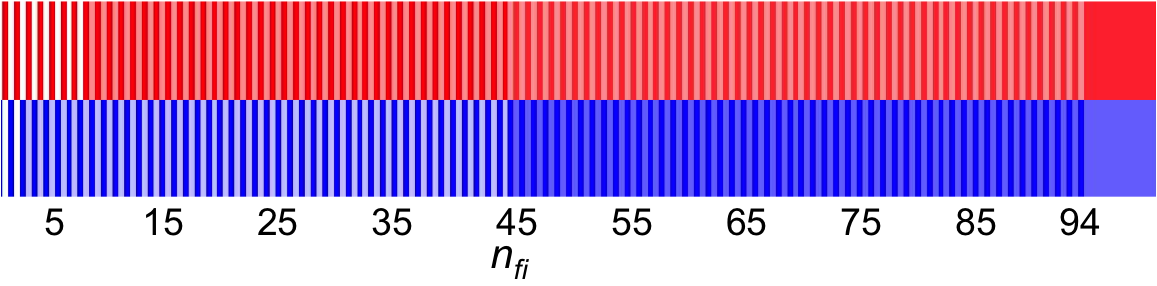
\includegraphics[width=0.85\linewidth]{TrainingData/figs/pt005proxdivAAO2.png} \\ 
(a) AAO approach with $\Delta=0.005$ \\ 
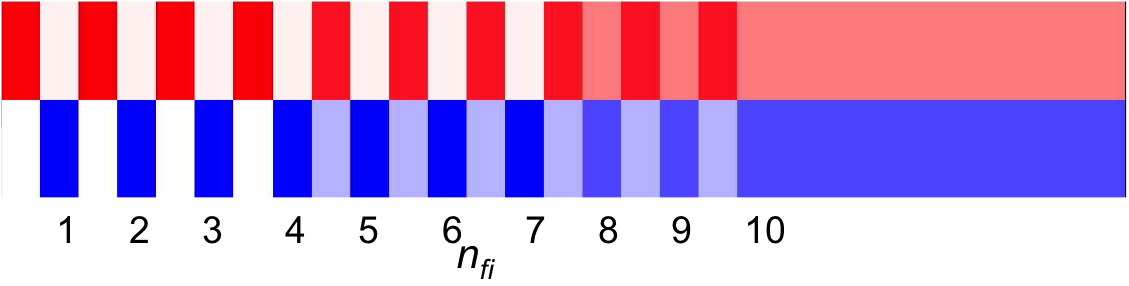
\includegraphics[width=0.85\linewidth]{TrainingData/figs/pt05proxdivAAO2.png} \\ 
(b) AAO approach with $\Delta=0.05$ \\ 
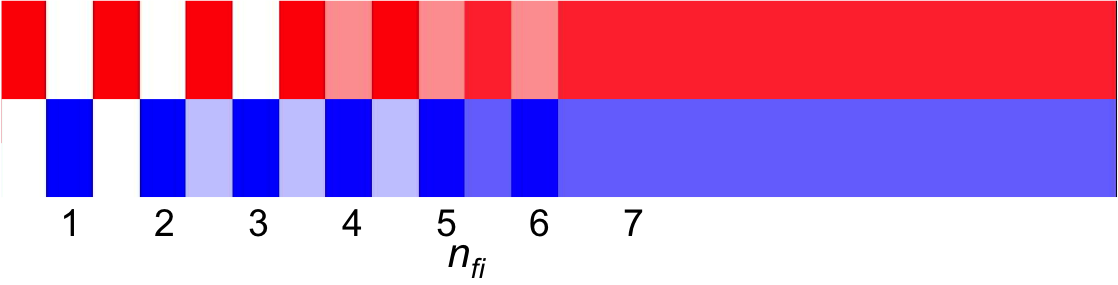
\includegraphics[width=0.85\linewidth]{TrainingData/figs/proxdivadaptAAO2.png} \\ 
(c) Adapt AAO approach 
\end{tabular} 
\caption[Variation in average proximity (red) and diversity (blue) of selected keywords for selecting 5 SRKs from 20 valid keywords of category ``$Baby$" using (a)  AAO with $\Delta=0.005$, (b) AAO with $\Delta=0.05$, and (c) Adapt AAO. ]{Variation in average proximity (red) and diversity (blue) of selected keywords for selecting 5 SRKs from 20 valid keywords of category ``$Baby$" using (a)  AAO with $\Delta=0.005$, (b) AAO with $\Delta=0.05$, and (c) Adapt AAO. Higher color intensity corresponds to a higher value of the corresponding objective function. $T$ increases along the X axis. Note that the range of variation in the two colors are different, and for both colors, white is assigned to the lowest value of the corresponding objective function value observed during the optimization. }
\label{fig:proxdivVariationAAO}
\end{figure*}


Since too large or small values of $\Delta$ lead to issues such as bias between objective functions, and large number of iterations taken for AAO approach to converge, we propose an adaptive approach that eliminates the need to have a fixed $\Delta$. Instead, the proposed approach updates $T$ based on the \textit{weakest permitted} algorithm iteration in the previous framework iteration whenever it detects repetitions in the selected keywords. The weakest permitted algorithm iteration is the algorithm iteration of either \textit{Max-Proximity} or \textit{Max-Diversity} with the least relative benefit that occurred in the previous framework iteration. Relative benefit has been defined for \textit{Max-Proximity} and \textit{Max-Diversity} algorithms in Section~\ref{sec:aaoproxmax} and Section~\ref{sec:aaodivmax} respectively. The adaptive annealing based alternating optimization (Adapt AAO) framework is presented in Algorithm~\ref{algo:AdaptAAO}. $WI_{Proximity}$ and $WI_{Diversity}$ represent the strength of the weakest permitted algorithm iteration permitted in the \textit{Max-Proximity} and \textit{Max-Diversity} algorithms respectively. Details on how $WI_{Proximity}$ and $WI_{Diversity}$ are computed in their respective algorithms are provided in Algorithms~\ref{algo:maxproximity} and \ref{algo:maxdiversity} respectively. Repetitions are detected in Algorithm~\ref{algo:AdaptAAO} when a set of selected keywords had been selected in a previous framework iteration.  


Based on the Adapt AAO approach, Fig.~\ref{fig:proxdivVariationAAO}(c) shows that the number of iterations taken to converge is much lower than in the case of $\Delta=0.005$ (Fig.~\ref{fig:proxdivVariationAAO}(a)). The resulting set of keywords is the same as in the case of $\Delta=0.005$, but with substantial reduction in number of iterations taken to converge (94 to 7). Since the Adapt AAO approach converges in significantly less framework iterations as compared to AAO, and does not result in any artificial bias towards an objective function, we only provide performance results based on Adapt AAO approach in Section~\ref{sec:expt}. 

\textbf{Complexity analysis for Algorithm~\ref{algo:AdaptAAO}.}
The \textit{Max-Proximity} algorithm (Algorithm~\ref{algo:maxproximity}) and the \textit{Max-Diversity} algorithm (Algorithm~\ref{algo:maxdiversity}) have worst-case complexities of $O(L^2 N_{Valid})$.  and $O(mL.N_{Valid})$ respectively. In each framework iteration, the two algorithms are run in alternation. Since $m > N_{Valid} > L$, the dominating number of computations is due to the term $O(mL.N_{Valid})$. Thus the total worst case time complexity of Algorithm~\ref{algo:AdaptAAO} is $O(mL.N_{Valid}N_{FrameworkIter})$ where $N_{FrameworkIter}$ is the number of framework iterations. 


\section{Experimental Results}
\label{sec:expt}
This section discusses our experimental setup and provides performance evaluation of the proposed framework. We conduct our experiments on YouTube videos using the YouTube API. We have used Wikipedia Thesaurus API \cite{nakayama2007wikipedia} and Reverse Dictionary \cite{ReverseDictionary} as the sources of candidate keywords given the name of a category. The candidates for a category are made distinct by removing any repetitions. The classifier used is a linear Support Vector Machine (SVM). Performance is compared against baseline classifier, which is a linear SVM trained over videos retrieved by category names. Classification accuracy is taken to be the performance measure. Textual data for a video is obtained from the Title, Keywords, and Description in the corresponding webpage. Each video webpage is represented as a bag of word vector of normalized word counts. Textual vocabulary is created based on collecting unigrams that occur in more than 0.5\% of total video webpages in training data, and by removing stop words (such as \textit{it, a, or, was} etc). \\
\indent      We conducted a user study to obtain videos viewed by a set of volunteers. More than 14000 videos viewed by 30 volunteers were collected. The testing videos for our proposed framework are obtained by manually labeling videos collected by the above user study. Testing videos for a category are also supplemented by videos from publicly available lists of popular (or useful or best) videos of the category.  \\
\indent      In the next three sub-sections, we summarize results of applying our proposed approach on three different sets of categories.
\begin{figure*}
%\setcaptionwidth{5.78cm}
\begin{minipage}[t]{0.45\textwidth}
\epsfig{width=6cm,height=4.0cm,figure=TrainingData/WIfigures/sears4_categoryName_vs_size_accuracyDiversity.eps}
%\vspace{-0.2in}
\caption{Classification accuracy and Intra-Category Diversity variation with number of training videos for baseline classifier}
\label{fig:searsCategoryName}
%\caption{Classification accuracy and Intra-Category Diversity (1) variation with number of training videos for baseline classifier}
\end{minipage}
\begin{minipage}[t]{0.45\textwidth}
\epsfig{width=6.5cm,height=4.0cm, figure=TrainingData/figs/sears4_all_vs_alpha_WIJ.eps}
%\vspace{-0.2in}
\caption{Classification accuracy variation for \{Baby, Clothing, Fitness, Food\} with respect to $\alpha$.  Dotted line shows baseline accuracy}
\label{fig:searsalpha}
%\caption{Classification accuracy variation for LCPD for \{Baby, Clothing, Fitness, Food\} with respect to $\alpha$.  Dotted line shows baseline accuracy}
\end{minipage}
\begin{minipage}[t]{0.45\textwidth}
\epsfig{width=6.5cm,height=4.0cm, figure=TrainingData/figs/sears4_vs_numkeywords_WIJ.eps}
%\epsfig{width=6.5cm,height=4.0cm, figure=TrainingData/WIfigures/sears4_vs_numkeywords_WIJ.eps}
%\vspace{-0.2in}
\caption{Classification accuracy variation for \{Baby, Clothing, Fitness, Food\} with respect to L}
\label{fig:searsNumkeywords}
%\caption{Classification accuracy variation for LCPD and Adapt AAO for \{Baby, Clothing, Fitness, Food\} with respect to L}
\end{minipage}
%\end{figure*}
%\begin{figure*}[htb!]
%\setcaptionwidth{5.78cm}
\begin{minipage}[t]{0.45\textwidth}
\epsfig{width=6cm,height=4.0cm, figure=TrainingData/figs/Jour_TimeKwdSelectSVMtrain2.eps}
%\epsfig{width=6cm,height=4.0cm, figure=TrainingData/WIfigures/Jour_TimeKwdSelectSVMtrain.eps}
%\epsfig{width=6cm,height=4.0cm, figure=TrainingData/WIfigures/Jour_TimeKwdSelectSVMtrain2.eps}
%\vspace{-0.2in}
\caption{Variation of time taken to select $L$ SRKs, and time taken to train linear SVM on obtained training data, with respect to $L$ }
\label{fig:searsTime}
\end{minipage}
\begin{minipage}[t]{0.45\textwidth}
\epsfig{width=6.5cm,height=4.0cm,figure=TrainingData/figs/musicGenre_all_vs_alpha_WIJ.eps}
%\vspace{-0.2in}
\caption{Classification accuracy variation for \{Classical music, Electronic Music, Jazz music, Rock music\} with respect to $\alpha$}
\label{fig:musicGenrealpha}
%\caption{Classification accuracy variation for LCPD for \{Classical music, Electronic Music, Jazz music, Rock music\} with respect to $\alpha$}
\end{minipage}
\begin{minipage}[t]{0.45\textwidth}
\epsfig{width=6.5cm,height=4.0cm, figure=TrainingData/figs/moviesGenre_all_vs_alpha_WIJ.eps}
%\vspace{-0.2in}
\caption{Classification accuracy  for \{Action movies, Comedy movies, Horror movies, Romantic movies\} with respect to $\alpha$}
\label{fig:movieGenrealpha}
%\caption{Classification accuracy  for LCPD for \{Action movies, Comedy movies, Horror movies, Romantic movies\} with respect to $\alpha$}
\end{minipage}
%\vspace{-0.15in}
\end{figure*}
%\vspace{-0.17in}
\begin{table}
\fontsize{8pt}{1em}\selectfont
\begin{center}
\caption{{Summary of average classification accuracy obtained using Adapt AAO approach}
\label{tab:SumAAOResults}}
\begin{tabular}{|p{0.25\linewidth}|p{0.20\linewidth}|p{0.20\linewidth}|p{0.20\linewidth}|}
		\hline
		\textbf{Approach to select L SRKs} & \textbf{Retail Product categories: Baby, Clothing, Fitness, Food} & \textbf{Genres of Music: Classical, Electronic, Jazz, Rock} & \textbf{Genres of Movies: Action, Comedy, Horror, Romantic} \\
		\hline
		Maximize average Proximity  & 91\%  & 91\% & 58.3\%  \\
		\hline
		Maximize diversity & 79.4\% & 89.7\%  &  48\%  \\
		\hline
		Based on Algorithm V & 92.6\%  & 92.4\% & 61.4\%  \\
		\hline
\end{tabular}
\end{center}
\end{table}

\subsection{Retail Product categories: Baby, Clothing, Fitness, Food }
%\vspace{-2mm}
     As discussed earlier, for a retail or department store (such as Walmart or Sears), knowledge of user preferences in product categories like the above is very useful. We first discuss results obtained using the baseline classifier followed by results obtained using the proposed approaches. 

Fig.~\ref{fig:searsCategoryName} shows the performance of the baseline classifier for classifying 255 test videos. It is seen that the performance of the baseline classifier improves initially as more videos are retrieved by category name and used for training. As shown in Fig.~\ref{fig:searsCategoryName}, the average (across all categories) Intra-Category Diversity (\ref{eq:diversityeqn}) of the training data thus obtained, increases with the number of retrieved videos, initially leading to performance improvement. However, as more videos are retrieved using the category name, the quality of retrieved videos by the video search engine begins degrading, and more training videos unrelated to the respective categories are retrieved and selected in their training data. This is reflected in loss in classification performance (around 700-800 videos per category) as more videos are retrieved using category name. In our experiments, 1000 videos are retrieved per SRK. In order to provide a fair comparison of our approach with the baseline, the number of training videos in both cases should be equal. However, from the trend in Fig.~\ref{fig:searsCategoryName} it can be seen that the best baseline performance is around 82.3\%. Since the YouTube API limits number of retrieved videos per keyword to 1000, we utilize the best classification performance (82.3\%) of baseline to compare with our techniques.  

In Fig.~\ref{fig:searsalpha}, we present performance variation of the proposed approaches with the moderation factor $\alpha$. Keywords from \cite{nakayama2007wikipedia} and top 200 keywords from \cite{ReverseDictionary}  are used as candidates, giving a total of 230 candidates per category. The number of valid keywords found per category are Baby: 81, Clothing: 63, Fitness: 78, Food: 52. The coefficients $N_1$ and $N_2$ in (\ref{eq:SRTeq}) are chosen such that $N_1$=$\frac{1}{N_2}$=$div(RV(C_i))$. Fig.~\ref{fig:searsalpha} shows the performance when $L$' number of SRKs are selected per category, where $L$' is the minimum number of valid keywords across all categories (which is 52 in this case). We show the performance using both Weighted Instances and Non-weighted Instances methods for LCPD. Weighted support vector machine \cite{yang2007weighted} is used to give varying weights to the training videos as per the Weighted Instances method. Fig.~\ref{fig:searsalpha} also shows the performance obtained by the Adapt AAO approach. As mentioned earlier, the performance of the Adapt AAO approach is same as that of the AAO approach with a small $\Delta$, and so we have only provided performance results of the former. For LCPD, $\alpha$ = 0.6 to 1 performs best for Non-weighted Instances method, and $\alpha$ = 0.6 to 0.8 performs best for Weighted Instances method. We observe that the Weighted Instances method in general performs better than the Non-weighted Instances method, as discussed in Section~\ref{sec:lcpd}. Moreover, both the methods have significantly better accuracy than the baseline classifier accuracy of 82.3\% (shown by the dotted line in Fig.~\ref{fig:searsalpha}). For the baseline case, the Intra-Category Diversity values (\ref{eq:diversityeqn}) of the training data are  \{\textit{0.259, 0.247, 0.244, 0.243}\} corresponding to \{\textit{Baby, Clothing, Fitness, Food}\}. Compared to this, the Intra-Category Diversity after all 52 SRKs (for $\alpha$ = 0.6) are used to retrieve training videos for above categories are \{\textit{0.439, 0.418, 0.395, 0.359}\}. The average (taken across all categories) Intra-Category Diversity has increased from $0.248$ for baseline to $0.403$ with LCPD (for 52 SRKs per category, and $\alpha$ = 0.6). Consequently, the classifier performance has also increased from 82.3\% (baseline performance) to $91$\% (Non-Weighted Instances) and $93.7$\% (Weighted Instances), thus demonstrating that higher Intra-Category Diversity in training videos results in better performance of the trained classification model. The classification accuracy obtained using Adapt AAO is 92.6\%. Based on Fig.~\ref{fig:searsalpha} it can also be seen that unlike LCPD, the performance of Adapt AAO does not depend on $\alpha$. While the performance of Adapt AAO is lower than the best performance of LCPD, the difference is marginal. In addition, the performance of Adapt AAO is significantly higher than the baseline performance. 

Fig.~\ref{fig:searsNumkeywords} shows how the performance of the proposed approaches varies with respect to $L$, i.e., the number of SRKs. For LCPD, $\alpha$ is kept constant at $0.6$ for this experiment. As can be seen for LCPD approach, while the performance of the Non-Weighted Instances method starts decreasing after initially increasing with increasing $L$, the Weighted Instances method performs better, and continues its improving performance with increasing $L$. The Adapt AAO approach is seen to consistently provide high classification accuracy. In addition, Adapt AAO offers the advantage of not requiring tuning of the parameter $\alpha$ which may require human effort or the availability of a labeled validation set. Table~\ref{tab:SumAAOResults} shows the accuracy obtained as per the proposed Adapt AAO approach as well as the accuracy obtained when all SRKs are selected to maximize only one objective function as discussed in Section~\ref{sec:aao}. It can be seen that the performance of our approach outperforms selecting SRKs based on only one objective function, namely average proximity (\ref{eq:proximityscore}) or diversity (\ref{eq:divaao}). 

Fig.~\ref{fig:searsTime} shows the time taken by the LCPD and Adapt AAO approaches with respect to the number of SRKs selected (i.e., $L$). Conforming to the complexity discussion in Section~\ref{sec:selectionSRK}, the time taken to select $L$ SRKs varies as $O(L)$ when the number of candidates and the categories are fixed. Fig.~\ref{fig:searsTime} also shows the time taken by a linear SVM (LibLinear implementation of SVM) to train over the collected set of training videos. The time-taken to learn the classifier varies approximately as $O(L)$. 

For our MATLAB-based implementation, the system memory usage for LCPD approach was 4.46 GBs for selecting 52 SRKs from 230 candidate keywords for category $Baby$. Since the Adapt AAO approach does not need to store the representations of individual retrieved videos retrieved per keyword, like in LCPD approach, the memory requirement for Adapt AAO approach is only 411 MBs. Training of SVM using 1000 videos for each of 52 SRKs required 1.4GBs. The empirical results presented demonstrate the feasibility of our proposed approach in terms of space and time complexities. 

We next present experimental results for two more sets of categories and focus on the classifier performance. 

\subsection{Genres of Music: Classical, Electronic, Jazz, Rock}
We have chosen these categories keeping the requirements of a music recommendation system in mind. While there are several, and often subjective, categorizations possible within Music, we have chosen the above four categories since these cover most other categories, and are broad in the sense of ease of labeling by a human expert. Top 100 keywords from \cite{ReverseDictionary}   are used to obtain candidates for each category. 26 SRKs are selected per category. 290 test videos are used to test the performance of the baseline classifier and the proposed approaches. In Fig.~\ref{fig:musicGenrealpha}, we present performance of the proposed approaches. While the performance of LCPD varies with $\alpha$, it is seen that performance of classifier for $\alpha \ge$ 0.2 is almost the same. The Weighted Instances method is again seen to outperform the Non-Weighted Instances method for higher $\alpha$ values ($\alpha \ge$0.2), and both show significantly better accuracy (92.4\% and 91\% respectively) than the baseline classifier (77.9\%). For these categories, Adapt AAO provides as high classification accuracy (92.4\%) as LCPD when 26 SRKs are used. This demonstrates the efficacy of the Adapt AAO approach to achieve high performance without the requirement of $\alpha$. 

\subsection{Genres of Movies: Action, Comedy, Horror, Romantic}
We here provide results for a set of categories that might be of interest for a movie recommendation system. \cite{ReverseDictionary} is used to obtain Candidate Keyword for each category. A total of 223 test videos are used to assess performance. 18 SRKs are selected per category. Fig.~\ref{fig:movieGenrealpha} supports the observation made with the previous sets of categories. For LCPD, the Weighted Instances is seen to be better performing than Non-Weighted Instances and both methods show significantly improved performance (62.8\% and 59.6\% respectively) compared to performance of baseline classifier (41.2\%).  Adapt AAO leads to marginally worse performance than LCPD and achieves 61.4\% classification accuracy. Both LCPD and AAO approaches achieve significant improvements in predictive correctness as compared to the baseline approach. 

Based on the above experiments, it can be seen that the proposed approaches LCPD and Adapt AAO, both lead to significant improvement in classification performance compared to the baseline classifier. The performance of Adapt AAO is slightly worse than LCPD, however since the former does not depend on $\alpha$, Adapt AAO offers a convenient approach to obtain high classification accuracy without necessitating manually provided preferences for objective functions or requiring manual effort to label validation videos and tune $\alpha$. 

%\vspace{-0.15in}

\section{Conclusions}
\label{sec:conclusion}

We have proposed a fully-automated framework to obtain high quality training videos for any arbitrary set of categories, without the need for any manual labeling that is needed by most related approaches. We analyze properties of training data that lead to high performance of the trained classifier. Based on the above properties, we propose approaches for selecting keywords to retrieve training videos, on the basis of their proximity to the categories of interest, and the resulting diversity in the training data. The first approach (LCPD) leads to high classification accuracy, although requires a parameter representing preference for defined objective functions. The parameter can be obtained through manually provided preferences for the objective functions, or by using manually labeled validation videos for tuning. In order to avoid the manual effort, we also provide an annealing based alternating optimization framework (AAO) and propose its adaptive variant (Adapt AAO) to select keywords. Such an approach does not require the articulation of preferences in parameterized form, with the trade-off of some loss in classification accuracy as compared to the LCPD approach. Experimental results on several sets of categories show the effectiveness of the training videos obtained by the proposed approaches, hence making classification of videos watched by users to arbitrary set of categories feasible. Consequently, this work may enable new personalization applications by enabling identification of user preferences in a set of categories relevant to the application.

\textbf{Acknowledgements}: The research discussed in this chapter was supported by the UCSD Center for Wireless Communication and the UC Discovery Grant program. The chapter has been co-authored with Prof. Sujit Dey and has been published in IEEE Access. Parts of this chapter have also been published in IEEE Web Intelligence 2013 conference. Authors would like to acknowledge the discussions with Dr. Nitesh Shroff regarding Section~\ref{sec:aao}. 

